\documentclass[master,tocprelim]{cornell}
%
% tocprelim option must be included to put the roman numeral pages in the
% table of contents
%
% The cornellheadings option will make headings completely consistent with
% guidelines.
%
% This sample document was originally provided by Blake Jacquot, and
% fixed up by Andrew Myers.
%
%Some possible packages to include
\usepackage{amsmath}
\usepackage{amsthm}
\usepackage{amsfonts}
\usepackage{booktabs}       % professional-quality tables
\usepackage{graphicx,pstricks}
\usepackage{graphics}
\usepackage{moreverb}
\usepackage{epsfig}
\usepackage[hang]{caption}
\usepackage{subcaption}
\usepackage{txfonts}
\usepackage{palatino}
\usepackage[dvipsnames]{xcolor}
\usepackage{url}
\usepackage[linesnumbered,ruled,longend,commentsnumbered]{algorithm2e}
\usepackage{hyperref}
\hypersetup{
  colorlinks,
  citecolor=black,
  filecolor=black,
  linkcolor=blue,
  urlcolor=black
}

\providecommand{\alltoall}{\textsc{AllToAll}\xspace}
\newcommand{\sysname}{\emph{FlashDMoE}\xspace}
\newtheorem{theorem}{Theorem}[section]
\newtheorem{lemma}[theorem]{Lemma}
\newtheorem{definition}{Definition}[section]
\newtheorem{remark}{Remark}[section]
\newtheorem{example}{Example}[theorem]
%if you're having problems with overfull boxes, you may need to increase
%the tolerance to 9999
\tolerance=9999

\bibliographystyle{plain}
%\bibliographystyle{IEEEbib}

\renewcommand{\caption}[1]{\singlespacing\hangcaption{#1}\normalspacing}
\renewcommand{\topfraction}{0.85}
\renewcommand{\textfraction}{0.1}
\renewcommand{\floatpagefraction}{0.75}

\title {OS Inspired Complete Kernel Fusion}
\author {Osayamen Jonathan Aimuyo}
\conferraldate {August}{2025}
\degreefield {Master of Science}
\copyrightholder{Osayamen Jonathan Aimuyo}
\copyrightyear{2025}

\begin{document}

\maketitle
\makecopyright
%! Author = jonathan
%! Date = 5/25/25
\begin{abstract}
    Your abstract goes here. Make sure it sits inside the brackets. If not,
    your biosketch page may not be roman numeral iii, as required by the
    graduate school.
\end{abstract}
%! Author = jonathan
%! Date = 5/25/25
\begin{biosketch}
Osayamen Jonathan Aimuyo is a computer science researcher interested in distributed and parallel computing systems
and algorithms; specifically, he seeks to address computational and communication bottlenecks in
large-scale machine learning execution on accelerators.
He earned a BS in computer engineering, \textit{summa cum laude}, with Tau Beta Pi and Phi Kappa Phi Honors from the
University of Texas at Dallas (class of 2023),
where he was a Presidential Achievement Scholar and a semifinalist
for the national Jack Kent Cooke Transfer Scholarship (2019).
He is currently a second-year CS MS student at Cornell University,
advised by Dr. Rachee Singh.
In industry, he contributed to large-scale distributed systems through internships at
Microsoft (\('22\) - \('24\)), Chime Financial ('22), and JPMorgan Chase (\('20\) - \('21\)).
Upon graduating from Cornell, he will intern at NVIDIA with the CUDA Math Libraries team,
before commencing his Computer Science PhD at Stanford University in Autumn 2025, where his research
would be supported by the \textbf{NSF GRFP} (2025) fellowship.
\end{biosketch}
%! Author = jonathan
%! Date = 5/25/25
\begin{dedication}
    \textit{To those who stubbornly refuse to give up despite circumstances suggesting otherwise.}
\end{dedication}

\begin{acknowledgements}
    First and foremost, I thank God, the Author of all things good,
    for sustaining me through every moment of this journey.
    He remained faithful in seasons of clarity and in shadows of doubt.
    Whatever merit this work holds is but a fragment of the grace I have received.

    To my advisor, \textbf{Dr. Rachee Singh}, thank you for the trust, the freedom, and the unwavering support!
    You gave me the space to think creatively, and your mentorship has been a true gift.
    I am especially grateful for your generosity, both professionally and personally.
    Your unique willingness to support your students holistically has
    helped me blossom as a well-rounded researcher.
    I also appreciate the lab resources (especially the GPUs) you made readily accessible.
    Much of the preliminary exploration and hypothesis testing for this research took place on them,
    and they contributed immense value to this thesis.

    To my minor field member, \textbf{Dr. Giulia Guidi}, thank you for being an excellent mentor
    and for your generosity with time and resources.
    Your provision of high-performance computing infrastructure made a tangible difference in this work,
    and I recognize the immense privilege it is to have had access to such powerful systems.

    To my second minor field member, \textbf{Dr. Chris De Sa}, I am deeply grateful for the opportunity to
    have learned Machine Learning Systems (MLSys) from you.
    Your passion and enthusiasm for the field is infectious, and your teaching is exceptional.
    If I could take your MLSys class again, I would in a heartbeat!

    To the \textbf{Christ Chapel Choir (’24/25)}, thank you for being my second family away from home.
    I joined you not knowing how to read sheet music, yet you welcomed me warmly and gave me room to grow rapidly.
    That kindness means more to me than I can express.
    One of my fondest memories was singing Handel’s \textit{Hallelujah Chorus} together; it was both exhilarating
    and quite fun!
    I am especially thankful to Dr.\ Art Ostrander (Choir Director) for his technical precision and leadership;
    Carrie Ostrander (Soprano);
    Dr.\ Deborah Martin (Alto and pianist);
    Jyying Juliana Kan (Soprano); Dr. Edwin Kan (Tenor);
    Margaret Brodhead (Pianist); Jim and Cindy Van Duren (Bass and Soprano);
    Amy Blumenthal (Alto); and Debbie Axtell (Alto).
    You have all helped shape the slightly more competent musician and vocalist I am today.

    To my colleagues at Cornell who made this journey richer:
    the CS MS classes of ’24 and ’25, Dr.\ Singh’s research group,
    Julian Bellavita, and the broader systems community, thank you for the fun events, collaboration, and conversation.

    Finally, to my parents—your quiet strength and
    unwavering support have been immeasurably valuable to all my academic endeavors.
    I would not be here without you.
    Thank you.
\end{acknowledgements}

\contentspage
\tablelistpage
\figurelistpage

\normalspacing \setcounter{page}{1} \pagenumbering{arabic}
\pagestyle{cornell} \addtolength{\parskip}{0.5\baselineskip}
%! Author = jonathan
%! Date = 5/26/25
\chapter{Introduction}\label{ch:introduction}
State-of-the-art large language models (LLMs), including DeepSeek-v3~\cite{deepep}, LLama4~\cite{llama4},
DBRX~\cite{dbrx} and Snowflake Arctic~\cite{arctic}, have adopted the Mixture-of-Experts (MoE)
~\cite{DBLP:conf/iclr/ShazeerMMDLHD17}
architecture for its computational efficiency~\cite{pmlr-v162-rajbhandari22a} and reliable
performance across language modeling tasks~\cite{deepep, llama4, jiang2024mixtralexperts}.
\begin{figure}[!ht]
    \centering
    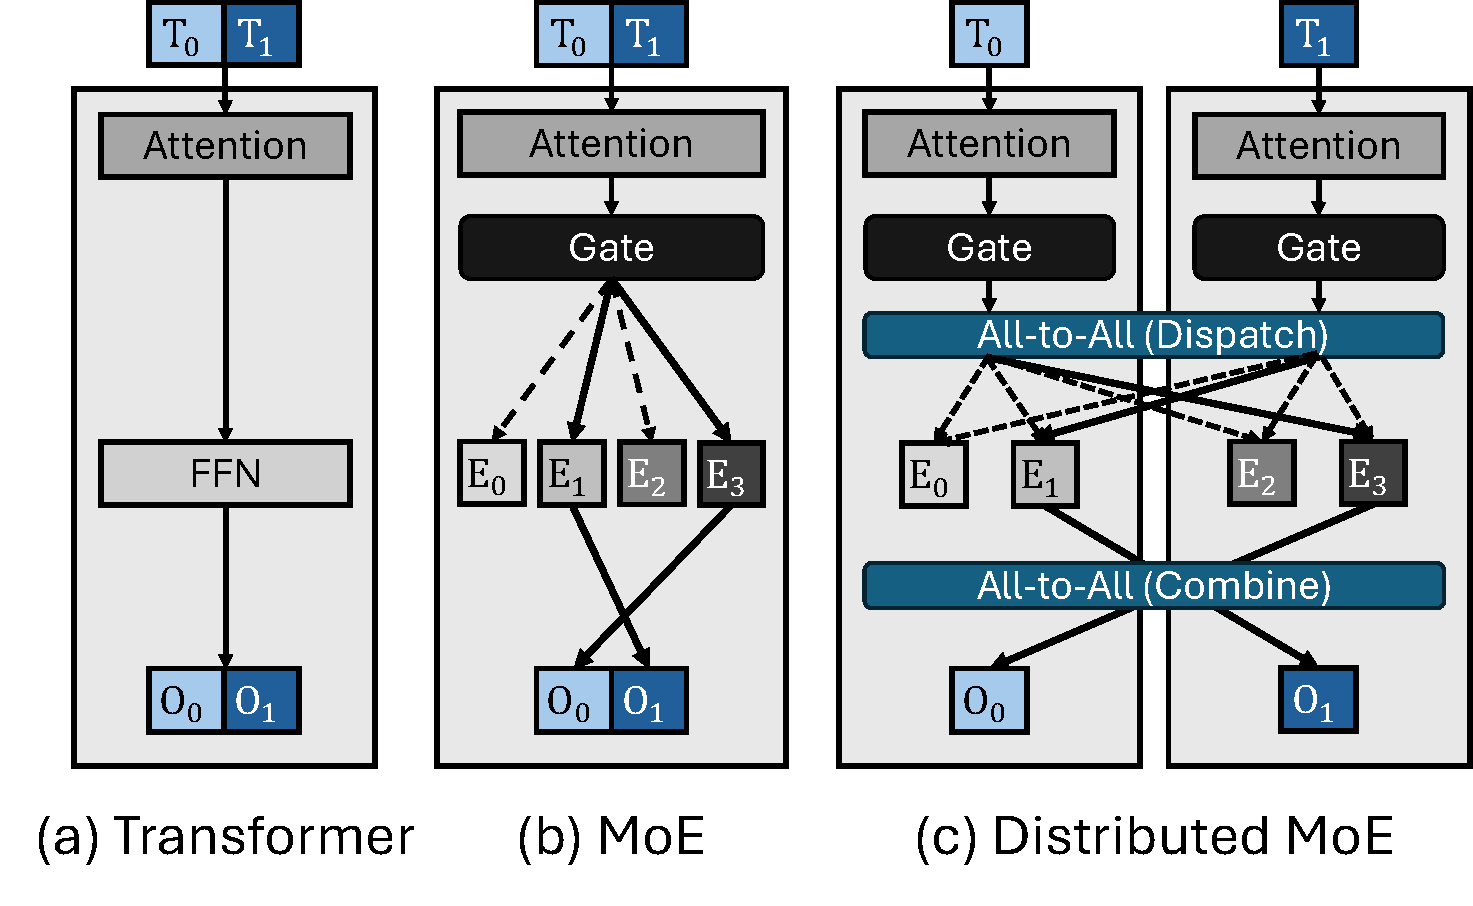
\includegraphics[width=0.55\textwidth, keepaspectratio]{figures/fig-bg-moe}
    \caption{Transformer blocks (a) without MoE, (b) with MoE, and (c) with distributed MoE and expert parallelism.
        \texttt{T}, \texttt{E}, and \texttt{O} represent input tokens, experts, and output activations, respectively.}
    \label{fig:bg:moe}
\end{figure}

Depicted in Figure~\ref{fig:bg:moe}(a), the conventional Transformer block consists of
a self-attention module followed by a feed-forward network (FFN)~\cite{NIPS2017_3f5ee243}.
In contrast, MoE architectures replace this single FFN with identically sized FFNs,
otherwise known as experts, (Figure~\ref{fig:bg:moe}(b)).
A trainable neural network, known as a gate function, sparsely activates these experts by
dynamically routing input tokens to selected experts at runtime.
This increase in model parameters (more FFNs) improves model quality without a
\textit{corresponding increase in computational cost}.
\section{Computational Cost Equivalence}\label{sec:comoutational-cost-equivalence}
The preceding claim seems counterintuitive because \emph{shouldn't the increase in the number of experts
yield a proportional increase in the model's computational operations?}
The answer is no, due to how tokens are \emph{distributed} across experts in comparison to the singular FFN.
For example, consider a token matrix $T$ as defined below where $S$ is the sequence length and $H$
the embedding dimension.
\[
    T \in \mathbb{R}^{S \times H}
\]
The typical FFN operator, defined below,
\begin{equation}\label{eq:ffn}
\textrm{FFN}(x) = W_2 \cdot \phi(x W_1 + b_1) + b_2
\end{equation}
comprises two linear transformations on learnable weight matrices
$W_1\in \mathbb{R}^{H \times P}$, $W_2 \in \mathbb{R}^{P \times H}$ each followed by additions with bias terms
$b_1 \in \mathbb{R}^{1 \times P}$, $b_2 \in \mathbb{R}^{1 \times H}$ and separated by a
nonlinear activation $\phi$ (e.g., GELU~\cite{hendrycks2023gaussianerrorlinearunits} or
ReLU~\cite{10.5555/3104322.3104425}).
Here dimension $P$ is an intermediate projection for the FFN\@, typically $P = 4\cdot H$~\cite{NEURIPS2024_9f2b171f}.
If we define $\mathcal{F}_{FFN}$ as the \textbf{F}loating \textbf{P}oint \textbf{OP}erations (FLOPs)
needed to compute a forward pass of the FFN, then using Equation~\ref{eq:ffn} we have the resulting expression.
\begin{equation}\label{eq:flopsffn}
\mathcal{F}_{FFN} = \mathcal{F}_{L_0} + \mathcal{F}_{L_1}
\end{equation}
where $\mathcal{F}_{L_i}$ is the FLOPs cost for computing linear transformation $i$.
These linear transformations are \textbf{GE}neral \textbf{M}atrix \textbf{M}ultiplications (GEMMs).
We know that multiplying two matrices of sizes $(M, K)$ and $(K, N)$ demands $2MNK$ FLOPs,
therefore we can expand Equation~\ref{eq:flopsffn} as
\begin{equation}\label{eq:flopsffn2}
\mathcal{F}_{FFN} = 2SHP + 2SHP = 4SHP
\end{equation}

An MoE model differs from the dense transformer by \emph{restricting} the number of
tokens~\cite{DBLP:conf/iclr/LepikhinLXCFHKS21, MLSYS2023_5a54f793} routed to an FFN
(interchangeably called expert).
Specifically, for a model with $N_e$ experts, each expert has a fixed capacity for tokens $S_e$ defined as follows
\begin{equation}\label{eq:capacity}
S_e = \frac{S}{N_e}
\end{equation}
With the above, we can compute $\mathcal{F}_{MoE}$.
Intuitively, this quantity would be the aggregate of $\mathcal{F}_{{FFN}_j}$ where $j \in \{0, \cdots, N_e - 1\}$.
\begin{equation}\label{eq:flopsmoe}
\mathcal{F}_{MoE} = \sum\limits_{j = 0}^{N_e - 1}\mathcal{F}_{{FFN}_j}
\end{equation}
Observe that $\mathcal{F}_{{FFN}_j}$ is derivable from Equation~\ref{eq:flopsffn}
by replacing $S$ with $S_e$.
Applying this observation and evaluating~\ref{eq:flopsmoe} gives the below result
\begin{equation}\label{eq:flopsmoe2}
\mathcal{F}_{MoE} = N_e \cdot 4S_{e}HP
\end{equation}
Substituting with~\ref{eq:capacity}, yields the below which proves that the computational cost is equivalent
between the MoE and dense transformer models!
\begin{equation}\label{eq:equivalence}
\mathcal{F}_{MoE} = 4SHP = \mathcal{F}_{FFN}
\end{equation}
This relationship presents empirically as uniform latency when $N_e$
increases but only till a certain threshold.
Exceeding this limit causes the latency to increase proportionally;
existing work gives no explanation for this phenomenon, but we
hypothesize GPU L1/L2 cache thrashing to be the culprit.

\section{Communication Overheads in Distributed MoE}\label{sec:communication-overheads-in-distributed-moe}
\begin{figure}[!ht]
    \centering
    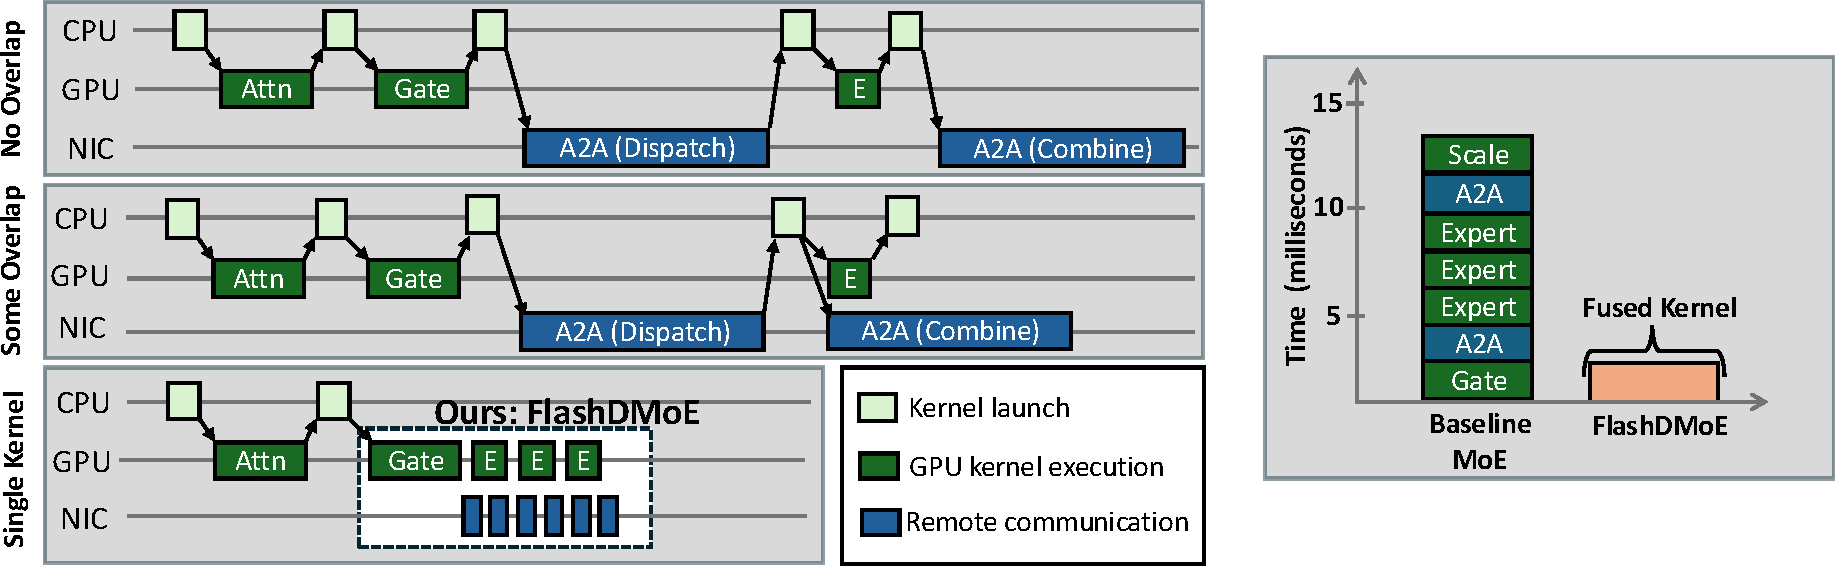
\includegraphics[width=0.98\textwidth, keepaspectratio]{figures/intro-fig}
    \caption{Comparing \sysname with state-of-the-art techniques that either do not overlap communication and
    computation (left, top) or do some overlap (left, middle). \sysname is a persistent kernel that fuses all
    computation and communication of the MoE operator (left, bottom). \sysname implements
    device-initiated computation (gate, expert FFN, scale) and communication tasks (right).}
    \label{fig:intro}
\end{figure}
As MoE model sizes grow, GPU memory constraints prevent hosting all experts on a single device.
The standard practice is to distribute experts across multiple GPUs using expert parallelism (EP),
which requires the gate function to route tokens via \alltoall communication
~\cite{deepep, arctic, dbrx, 10.1145/3577193.3593704}.
Overall, each MoE layer executes two \alltoall operations during inference,
introducing significant communication overhead. \alltoall communication is challenging to optimize on GPU networks
and is highly sensitive to straggler delays---a phenomenon where a single \emph{straggler} GPU delays
all others from making progress.
In practice, these communication operations can account for up to 40\% of the total runtime during inference or
training~\cite{10.1145/3603269.3604869, MLSYS2024_339caf45}.
\section{Kernel Launch Overheads in Distributed MoE}\label{sec:kernel-launch-overheads-in-distributed-moe}
\begin{table}[!ht]
    \centering
    \small
    \setlength{\tabcolsep}{8pt}
    \renewcommand{\arraystretch}{0.9}
    \begin{tabular}{@{}lc@{}}
        \toprule
        \textbf{Works} & \textbf{Launched GPU Ops} \\ \midrule
        \sysname & 1 \\
        COMET~\cite{comet} & 33 \\
        Megatron-LM CUTLASS~\cite{megatron, 10.1145/3458817.3476209} & 85 \\
        Megatron-LM TE~\cite{megatron, 10.1145/3458817.3476209} & 261 \\
        Megatron-LM + DeepEP~\cite{deepep} & 432 \\
        DeepSpeedMoE~\cite{pmlr-v162-rajbhandari22a} & 550 \\
        \bottomrule
    \end{tabular}
    \caption{\textbf{Kernel Fusion Comparison.}
    Our method is the first to fully fuse the DMoE layer into a single GPU kernel.
    We report GPU operations from detailed profiling with Nsight Systems.}
    \label{tab:gpuOps}
\end{table}
To mitigate these communication bottlenecks,
recent work pipelines computation with communication tasks
(Figure~\ref{fig:intro}, middle left).
However, the effectiveness of these solutions is limited by the overhead of
launching many kernels from the CPU\@.
Specifically, MoE layers interleave multiple computation kernels
(such as gate and expert computations) and communication operations,
forcing the CPU to launch many GPU kernels per forward pass
(see Table~\ref{tab:gpuOps}).
Frequent kernel launches negatively affect performance by:
(1) creating non-deterministic kernel start times across GPUs, exacerbating straggler issues;
(2) introducing unnecessary synchronization points,
causing GPUs to wait on peers or the CPU before proceeding;
and (3) incurring repeated global memory round trips at kernel boundaries.
Although CUDA graphs~\cite{cuda_graphs_nvidia_blog} can partially mitigate the
first issue in static workloads,
they are incompatible with MoE's dynamic expert routing patterns.
Addressing the remaining issues requires novel solutions,
which we provide in this work through complete kernel fusion and
asynchronous device-initiated communication.
\section{This work's Contributions: DMoE in a single kernel}\label{sec:contributions:-moe-operator-in-a-single-kernel}
To overcome these fundamental inefficiencies in state-of-the-art MoE models,
we develop \sysname, a novel MoE architecture that integrates all computation
and communication tasks into a single persistent GPU kernel, namely
a kernel that remains active for the entirety of the MoE operator
(Figure~\ref{fig:intro} bottom left).
Instead of multiple kernel launches coordinated by the CPU,
\sysname requires launching only one kernel,
significantly reducing the involvement of the CPU in the MoE operator.
Within the fused kernel, \sysname implements a concurrent-programming
model to achieve fine-grained parallelization
of computation and communication tasks of the MoE operator.
This design enables \sysname to efficiently utilize GPU resources by reducing idle time.
\subsection{Warp Specialization and Tile Parallelism.}\label{subsec:wstp}
\begin{figure}[!ht]
    \centering
    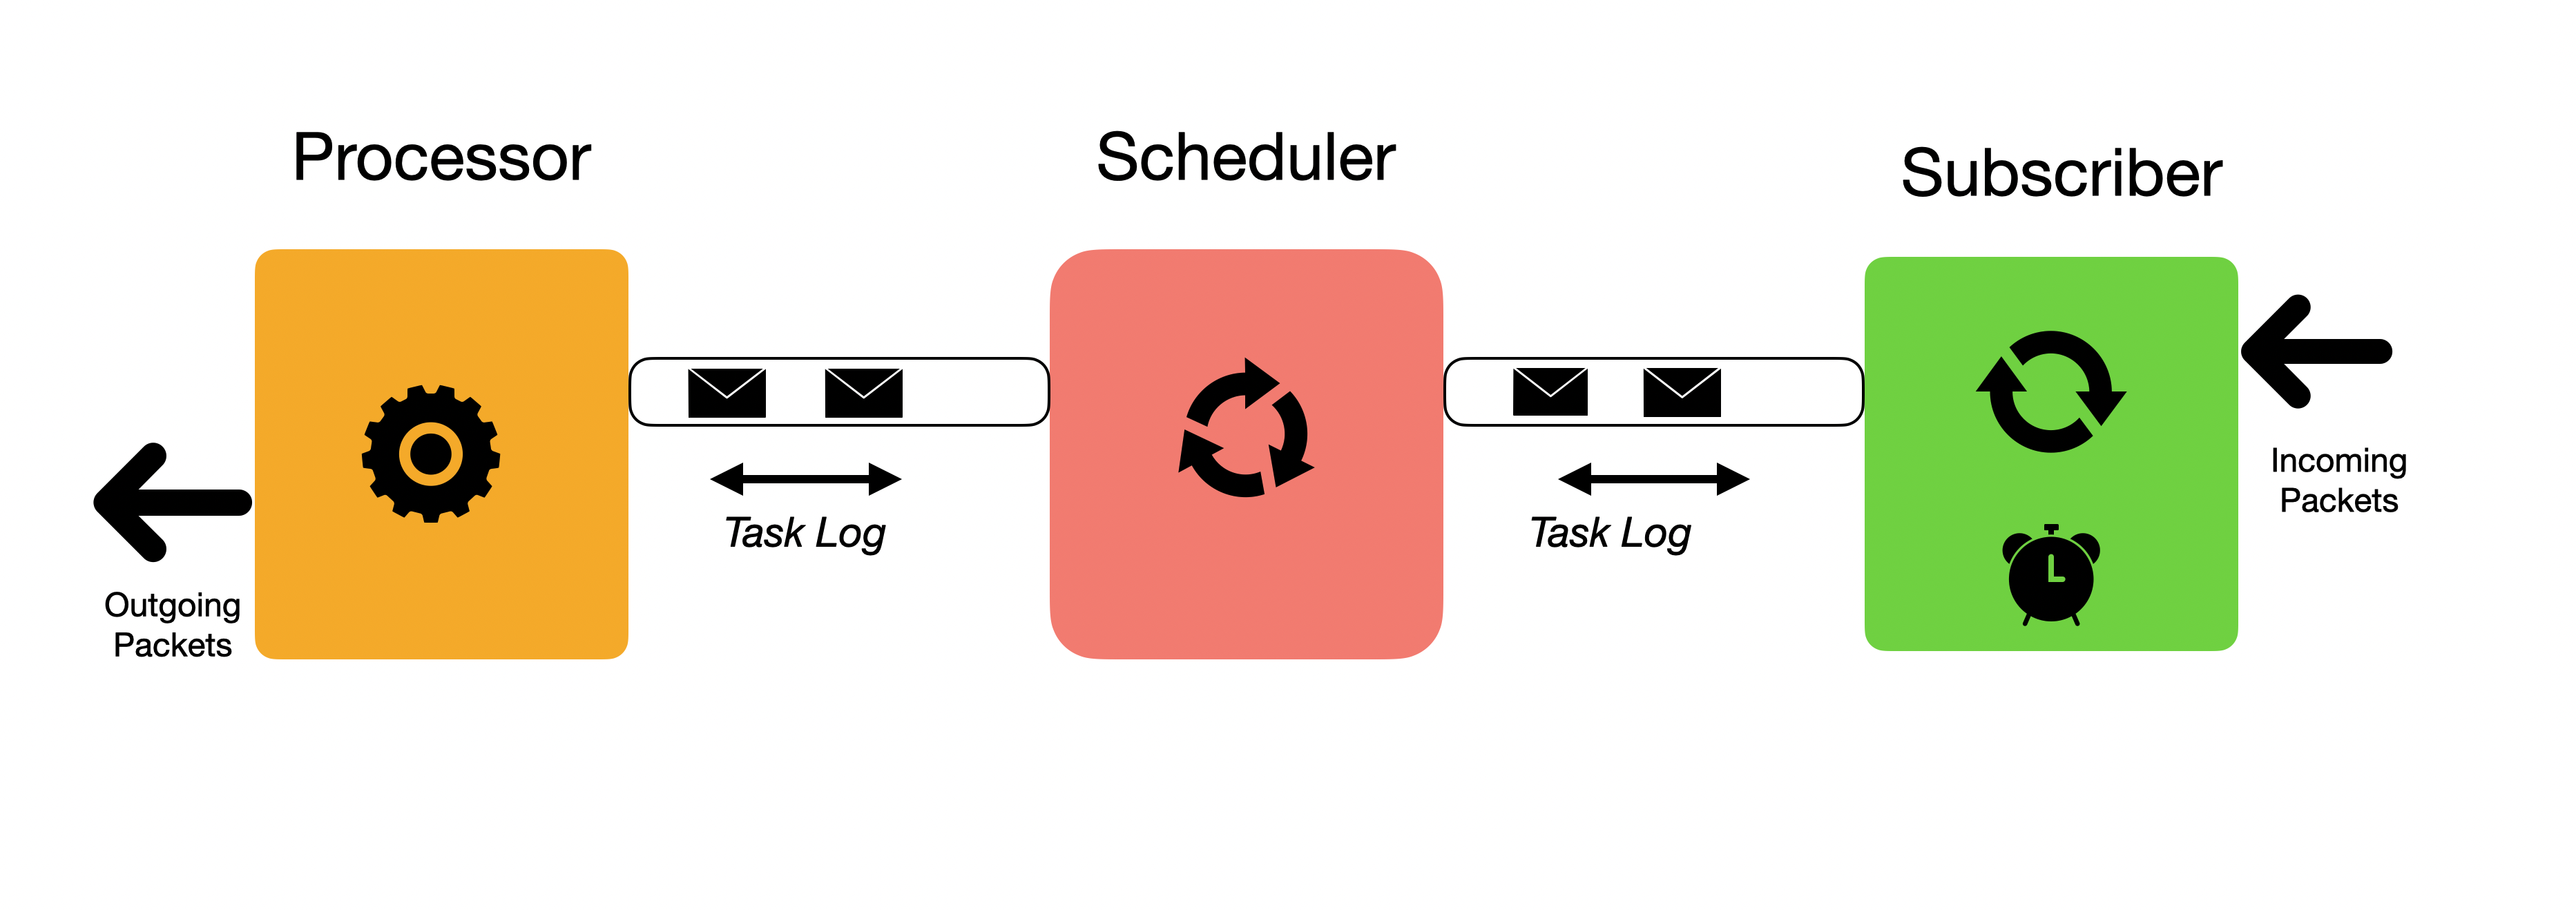
\includegraphics[width=0.98\textwidth, keepaspectratio]{figures/flash_actors}
    \caption{\sysname Actors. The \textcolor{LimeGreen}{Subscriber} observes received remote \emph{packets}
    (blob of tiles), decodes them into \emph{tasks} and notifies the scheduler of the enqueued tasks.
    We assign three CUDA warps to this role.
    The \textcolor{Salmon}{Scheduler} maintains a \emph{ready queue} of \textcolor{Orange}{Processors}
    from which it schedules tasks. The \textcolor{Yellow}{Processors} performs the operation encoded in its task
    descriptor and eagerly communicates its output, if necessary.}
    \label{fig:flash_actors}
\end{figure}
\sysname implements \emph{tile-level parallelism},
meaning it partitions input token matrices into smaller,
independent units called \emph{tiles},
which are processed concurrently by GPU thread warps.
These warps specialize as \emph{processors}
since they process input to compute the gate function and expert FFNs.
A handful of warps perform specialized administrative tasks of
(1) scheduling computational tasks by mapping them to warps (\emph{scheduler}), and
(2) communicating with other GPUs (\emph{subscriber}).
This design allows \sysname to dynamically assign tasks to GPU warps based
on warp availability and the current workload,
ensuring that no warp remains idle while useful work can be done.
\sysname selects tile dimensions to maximize GPU arithmetic intensity and
minimize register pressure.
\subsection{Asynchronous and payload-efficient communication.}\label{subsec:asynchronous-and-payload-efficient-communication.}
\begin{figure}[!ht]
    \centering
    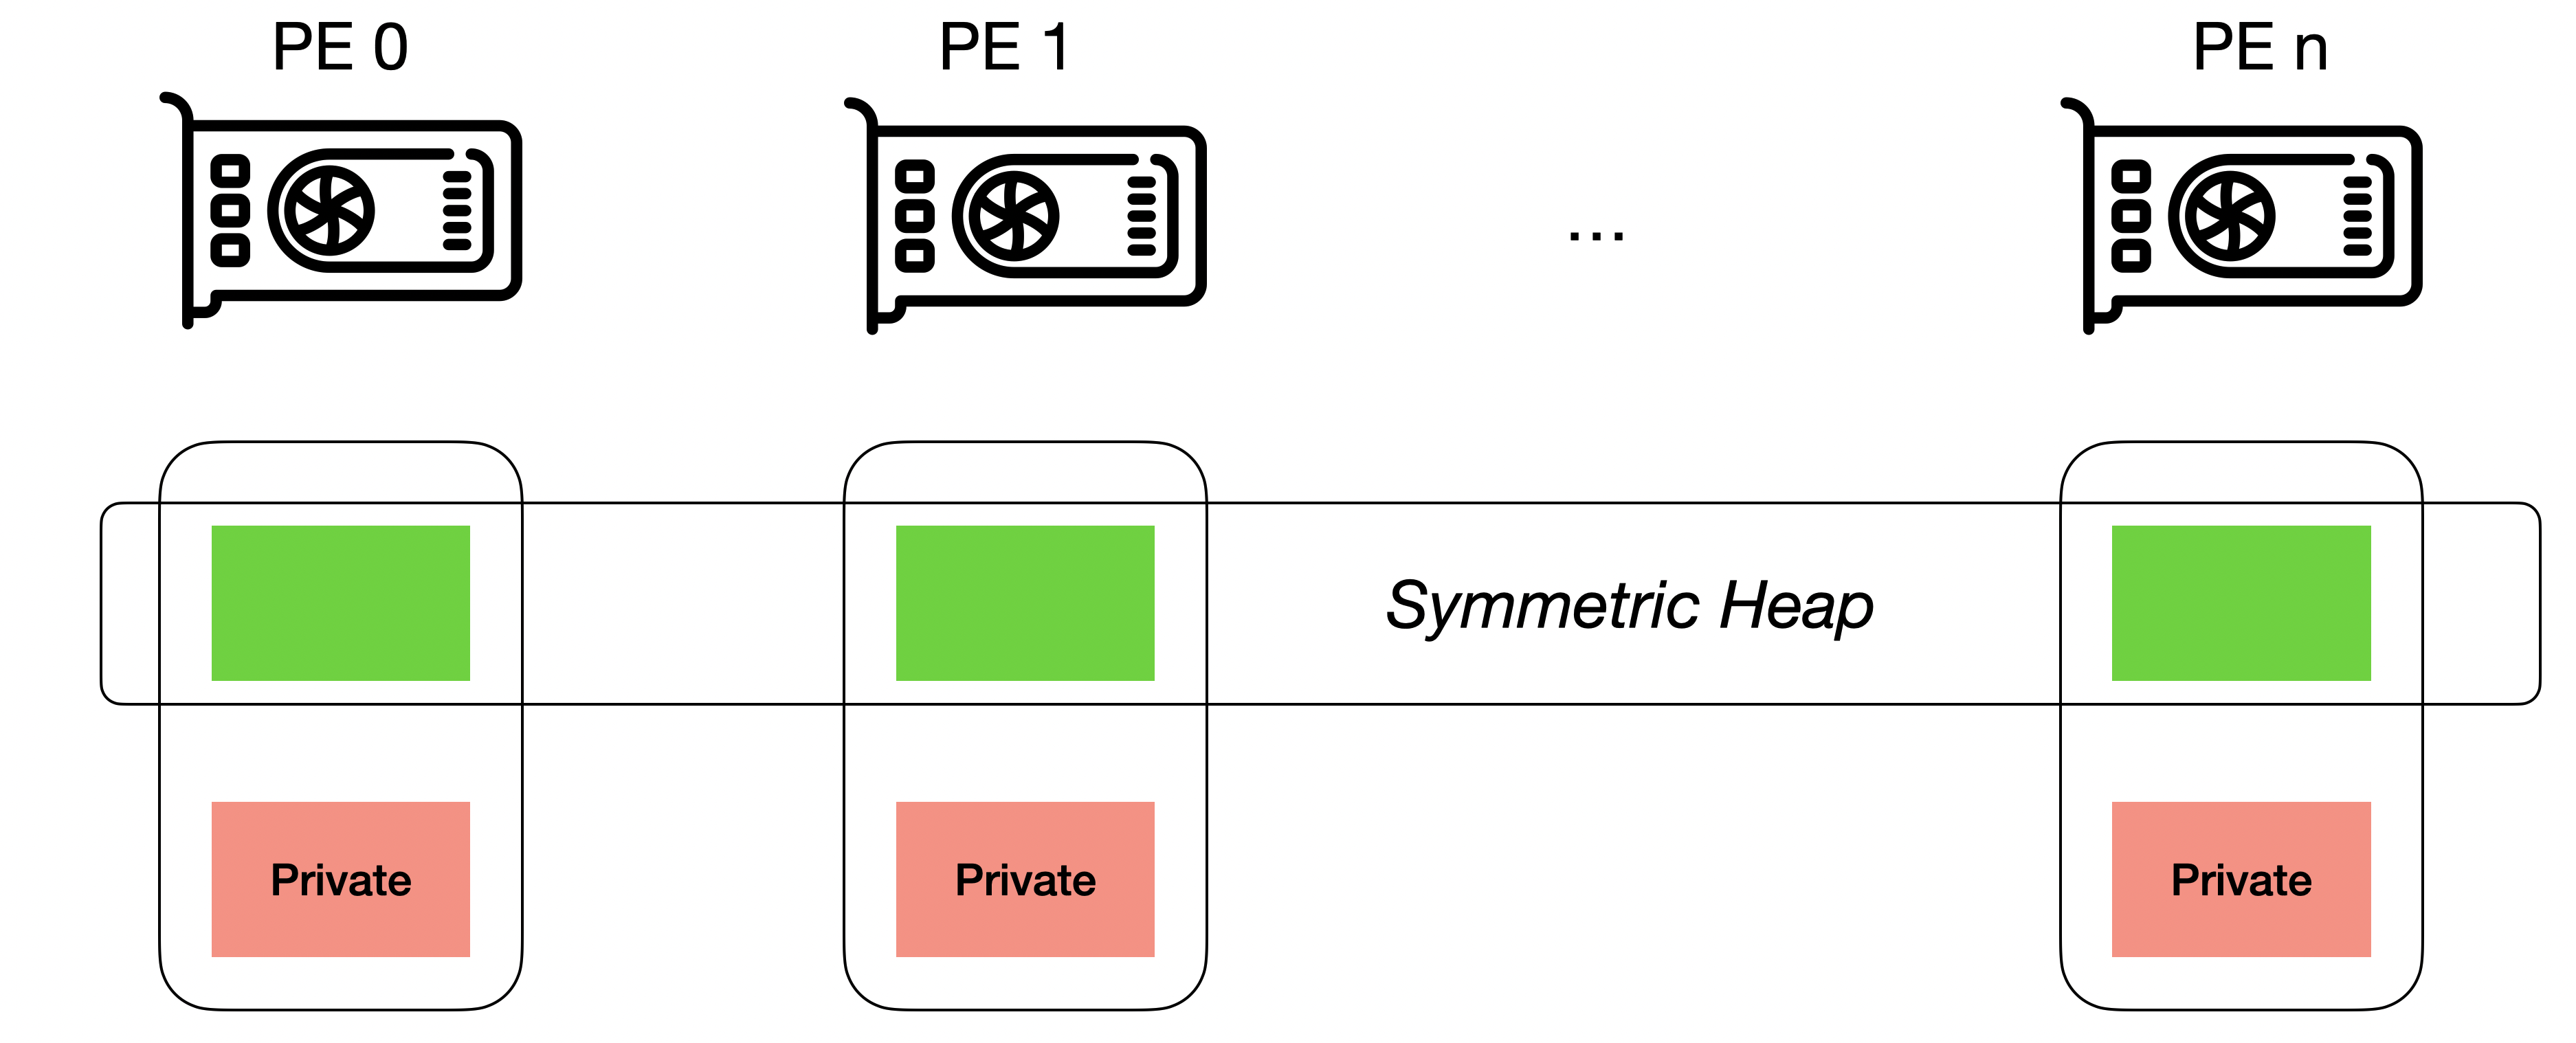
\includegraphics[width=0.98\textwidth, keepaspectratio]{figures/pgas}
    \caption{Depiction of a Partitioned Global Adress Space (PGAS)~\cite{10.1145/1278177.1278183}
        across a \textit{team} of \textbf{P}rocessing \textbf{E}lements (PEs). The symmetric heap is an
    unifromly sized memroy region resident on each PE and accessible by every other PE via one-sided
    \textbf{D}irect \textbf{M}emory \textbf{A}ccess (DMA) or \textbf{R}emote DMA (RDMA) operations.}
    \label{fig:pgas}
\end{figure}
By redesigning the MoE operator from the ground up,
\sysname resolves fundamental inefficiencies inherent
in the conventional MoE execution pipeline.
One inefficiency is due to workload imbalance across GPUs due to
skewed popularity of experts.
Existing implementations~\cite{pmlr-v162-rajbhandari22a} indiscriminately perform \alltoall communications,
transferring null values to GPUs that host unpopular experts,
resulting in wasted communication bandwidth and unnecessary computations on null matrices.
\sysname introduces \emph{payload-efficient} communication
by sending tokens only to GPUs with actively selected experts,
thereby conserving both communication and computational resources.
\subsection{Technical Challenges}\label{subsec:technical-challenges}
Realizing the single-kernel design of \sysname required solving several
technical challenges.
\sysname's design is a radical departure from
traditional synchronous \alltoall collectives,
where GPUs remain idle until the slowest GPU completes its communication.
Instead, \sysname establishes a global address space via NVSHMEM~\cite{nvshm} across all GPUs to
achieve asynchronous communication between GPUs while allowing them to
continue performing useful computation tasks.
To implement device-initiated computation primitives,
\sysname develops custom high-performance GEMM operations for the MoE operator in
CUTLASS~\cite{Thakkar_CUTLASS_2023}.
\subsection{Research Papers}\label{subsec:research-papers}
This thesis comprises a first-author publication~\cite{10.1145/3725536.3725539} at ACM SIGMETRICS'24 and another first-author
submission in review at NeurIPS \('25\).


%! Author = jonathan
%! Date = 5/26/25
\chapter{Related Work}\label{ch:related-work}
\noindent\textbf{Computation-Communication Overlap.}
To reduce the communication overheads of synchronization in distributed DNN training, many research efforts have been focused on
increasing the overlap of computation and communication.
For generic Transformer-based models without MoE layers,
many works~\cite{coconet,decomposition,centauri,t3,megascale,co2,syndicate,ccfuser,fused}
have provided insights and techniques to
partition and schedule computation and communication operations, a
imed at finer-grained overlapping.
To address the challenges posed by \alltoall communication and
expert parallelism in MoE training, Tutel~\cite{tutel} and FasterMoE~\cite{fastermoe}
overlap \alltoall with expert computation.
Lancet~\cite{lancet} additionally enables both non-MoE computation in
forward pass and weight gradient computation in backward pass to be overlapped with \alltoall.
Despite overlapping, the performance of these approaches is
limited in practice due to blocking synchronous collective communication with barriers.
In contrast, \sysname fundamentally
eliminates the inefficiencies with
asynchronous, device-initiated data transfers overlapped with tiled computation
all \emph{within a single kernel},
further differentiating itself from SOTA works~\cite{triton-dist, comet, deepep}
who also use this form of kernel-initiated communication but at a coarse-grained granularity
and without complete kernel fusion.
\chapter{Motivation}\label{ch:motivation}
\section{Straggler Effect}\label{subsec:straggler-effect}
\begin{figure}[!ht]
    \centering
     \begin{subfigure}{0.49\textwidth}
        \centering
        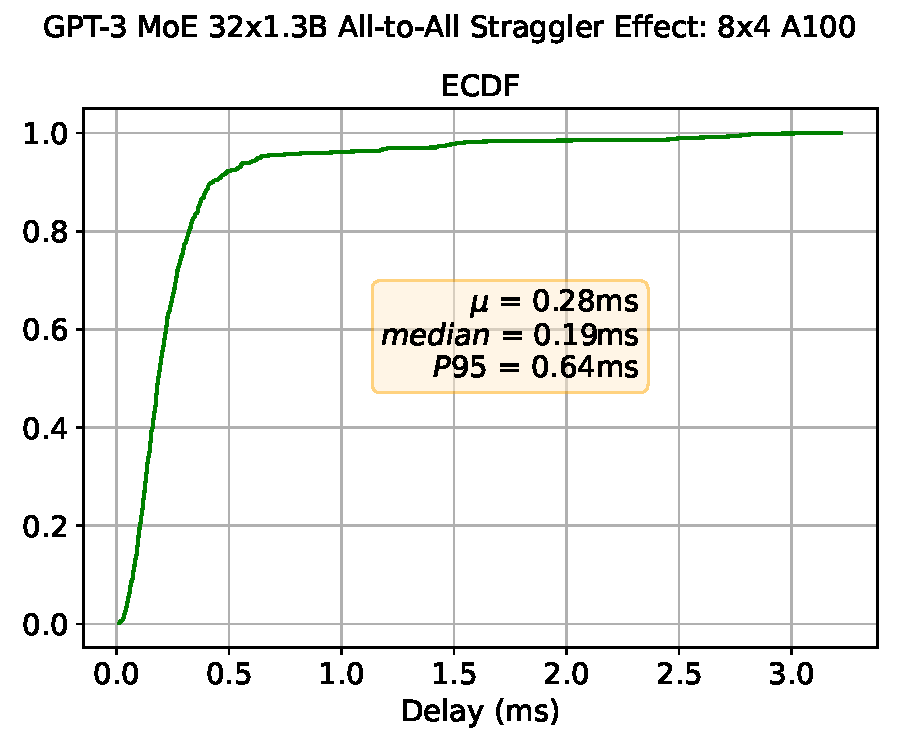
\includegraphics[width=\linewidth, keepaspectratio]{figures/GPT-3_MoE_32x1.3B_ecdf}
        \caption{ECDF}
        \label{sub:ecdf_perl}
    \end{subfigure}
    \begin{subfigure}{0.49\textwidth}
        \centering
        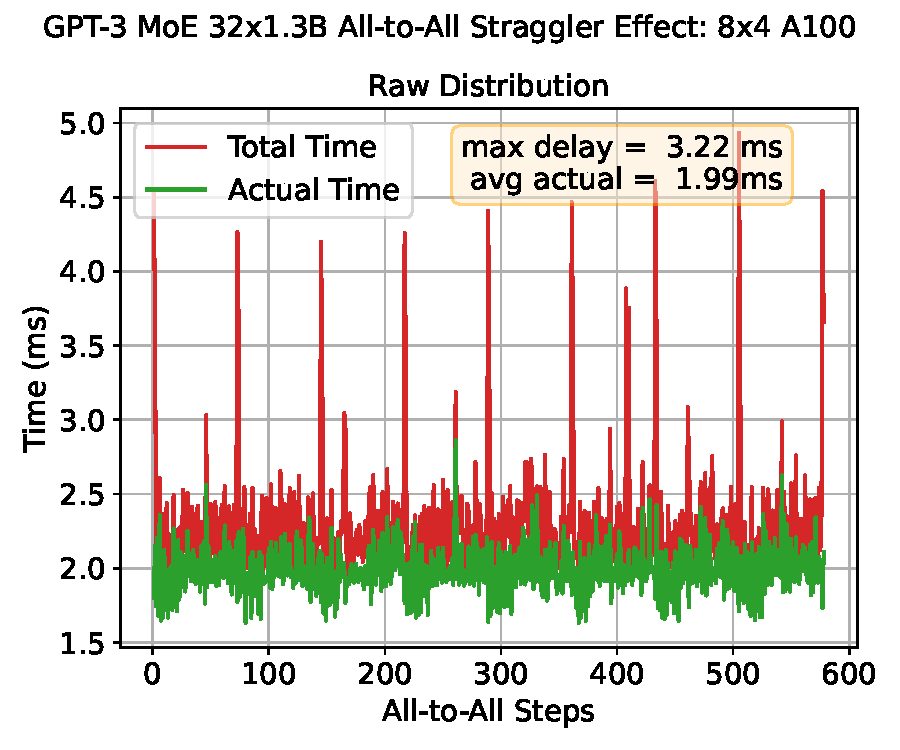
\includegraphics[width=\linewidth, keepaspectratio]{figures/GPT-3_MoE_32x1.3B}
        \caption{Raw Distribution}
        \label{sub:raw_perl}
    \end{subfigure}
    \vspace{1em} % space between rows
    \begin{subfigure}{0.49\textwidth}
        \centering
        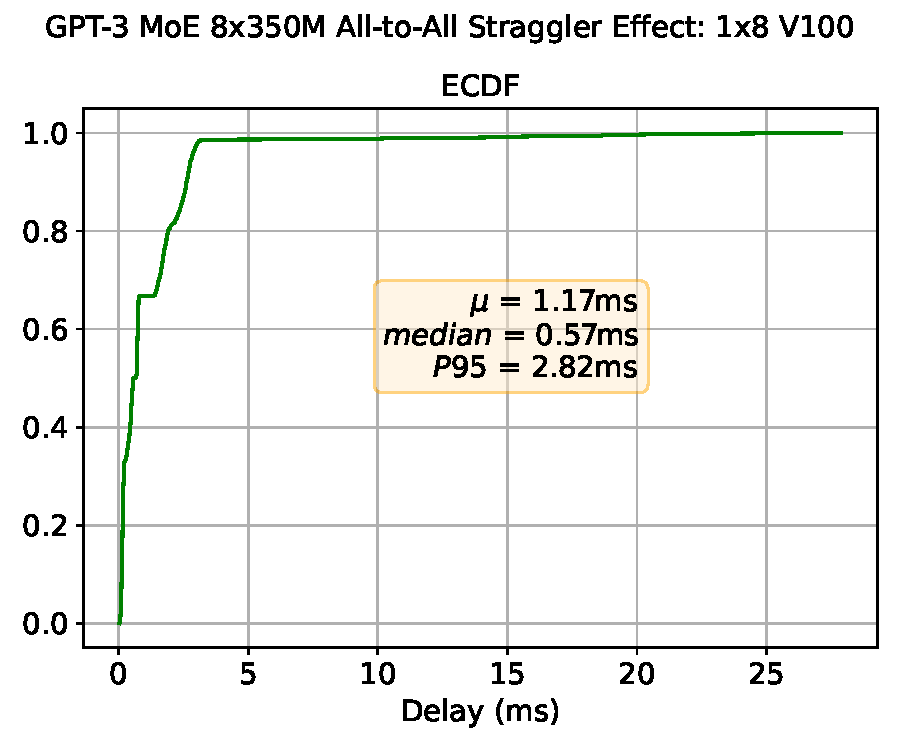
\includegraphics[width=\linewidth, keepaspectratio]{figures/GPT-3_MoE_8x350M_ecdf}
        \caption{ECDF}
        \label{sub:ecdf_az}
    \end{subfigure}
    \begin{subfigure}{0.49\textwidth}
        \centering
        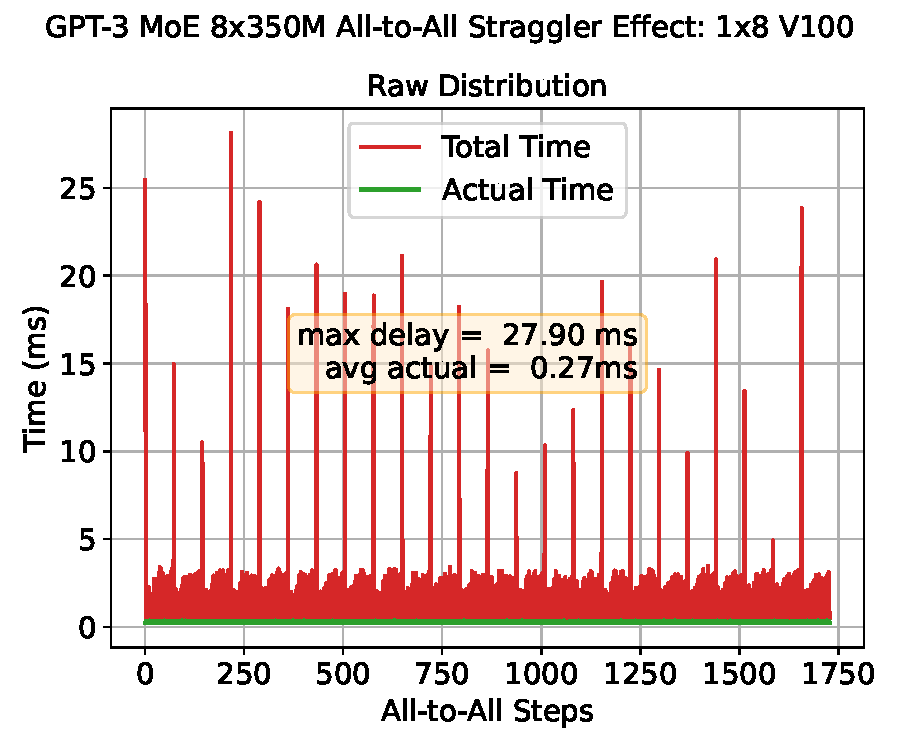
\includegraphics[width=\linewidth, keepaspectratio]{figures/GPT-3_MoE_8x350M}
        \caption{Raw Distribution}
        \label{sub:raw_az}
    \end{subfigure}
    \caption{Straggler effect of synchronous \alltoall. $M\times N$ A100 or V100 denotes
        $N$ GPUs within a node across $M$ nodes.
        Every GPU communicates with every other GPU per~\alltoall step.
        We capture the distribution of delay induced by stragglers across many steps.
        \textbf{Actual Time} $t_a$ denotes the fastest kernel execution time across all GPUs,
        conversely \textbf{Total Time} $t$ is the maximum recorded step time, while
        $Delay$ is the maximum difference between $t$ and $t_a$.}
    \label{fig:straggler}
\end{figure}
\begin{figure}[!ht]
    \centering
    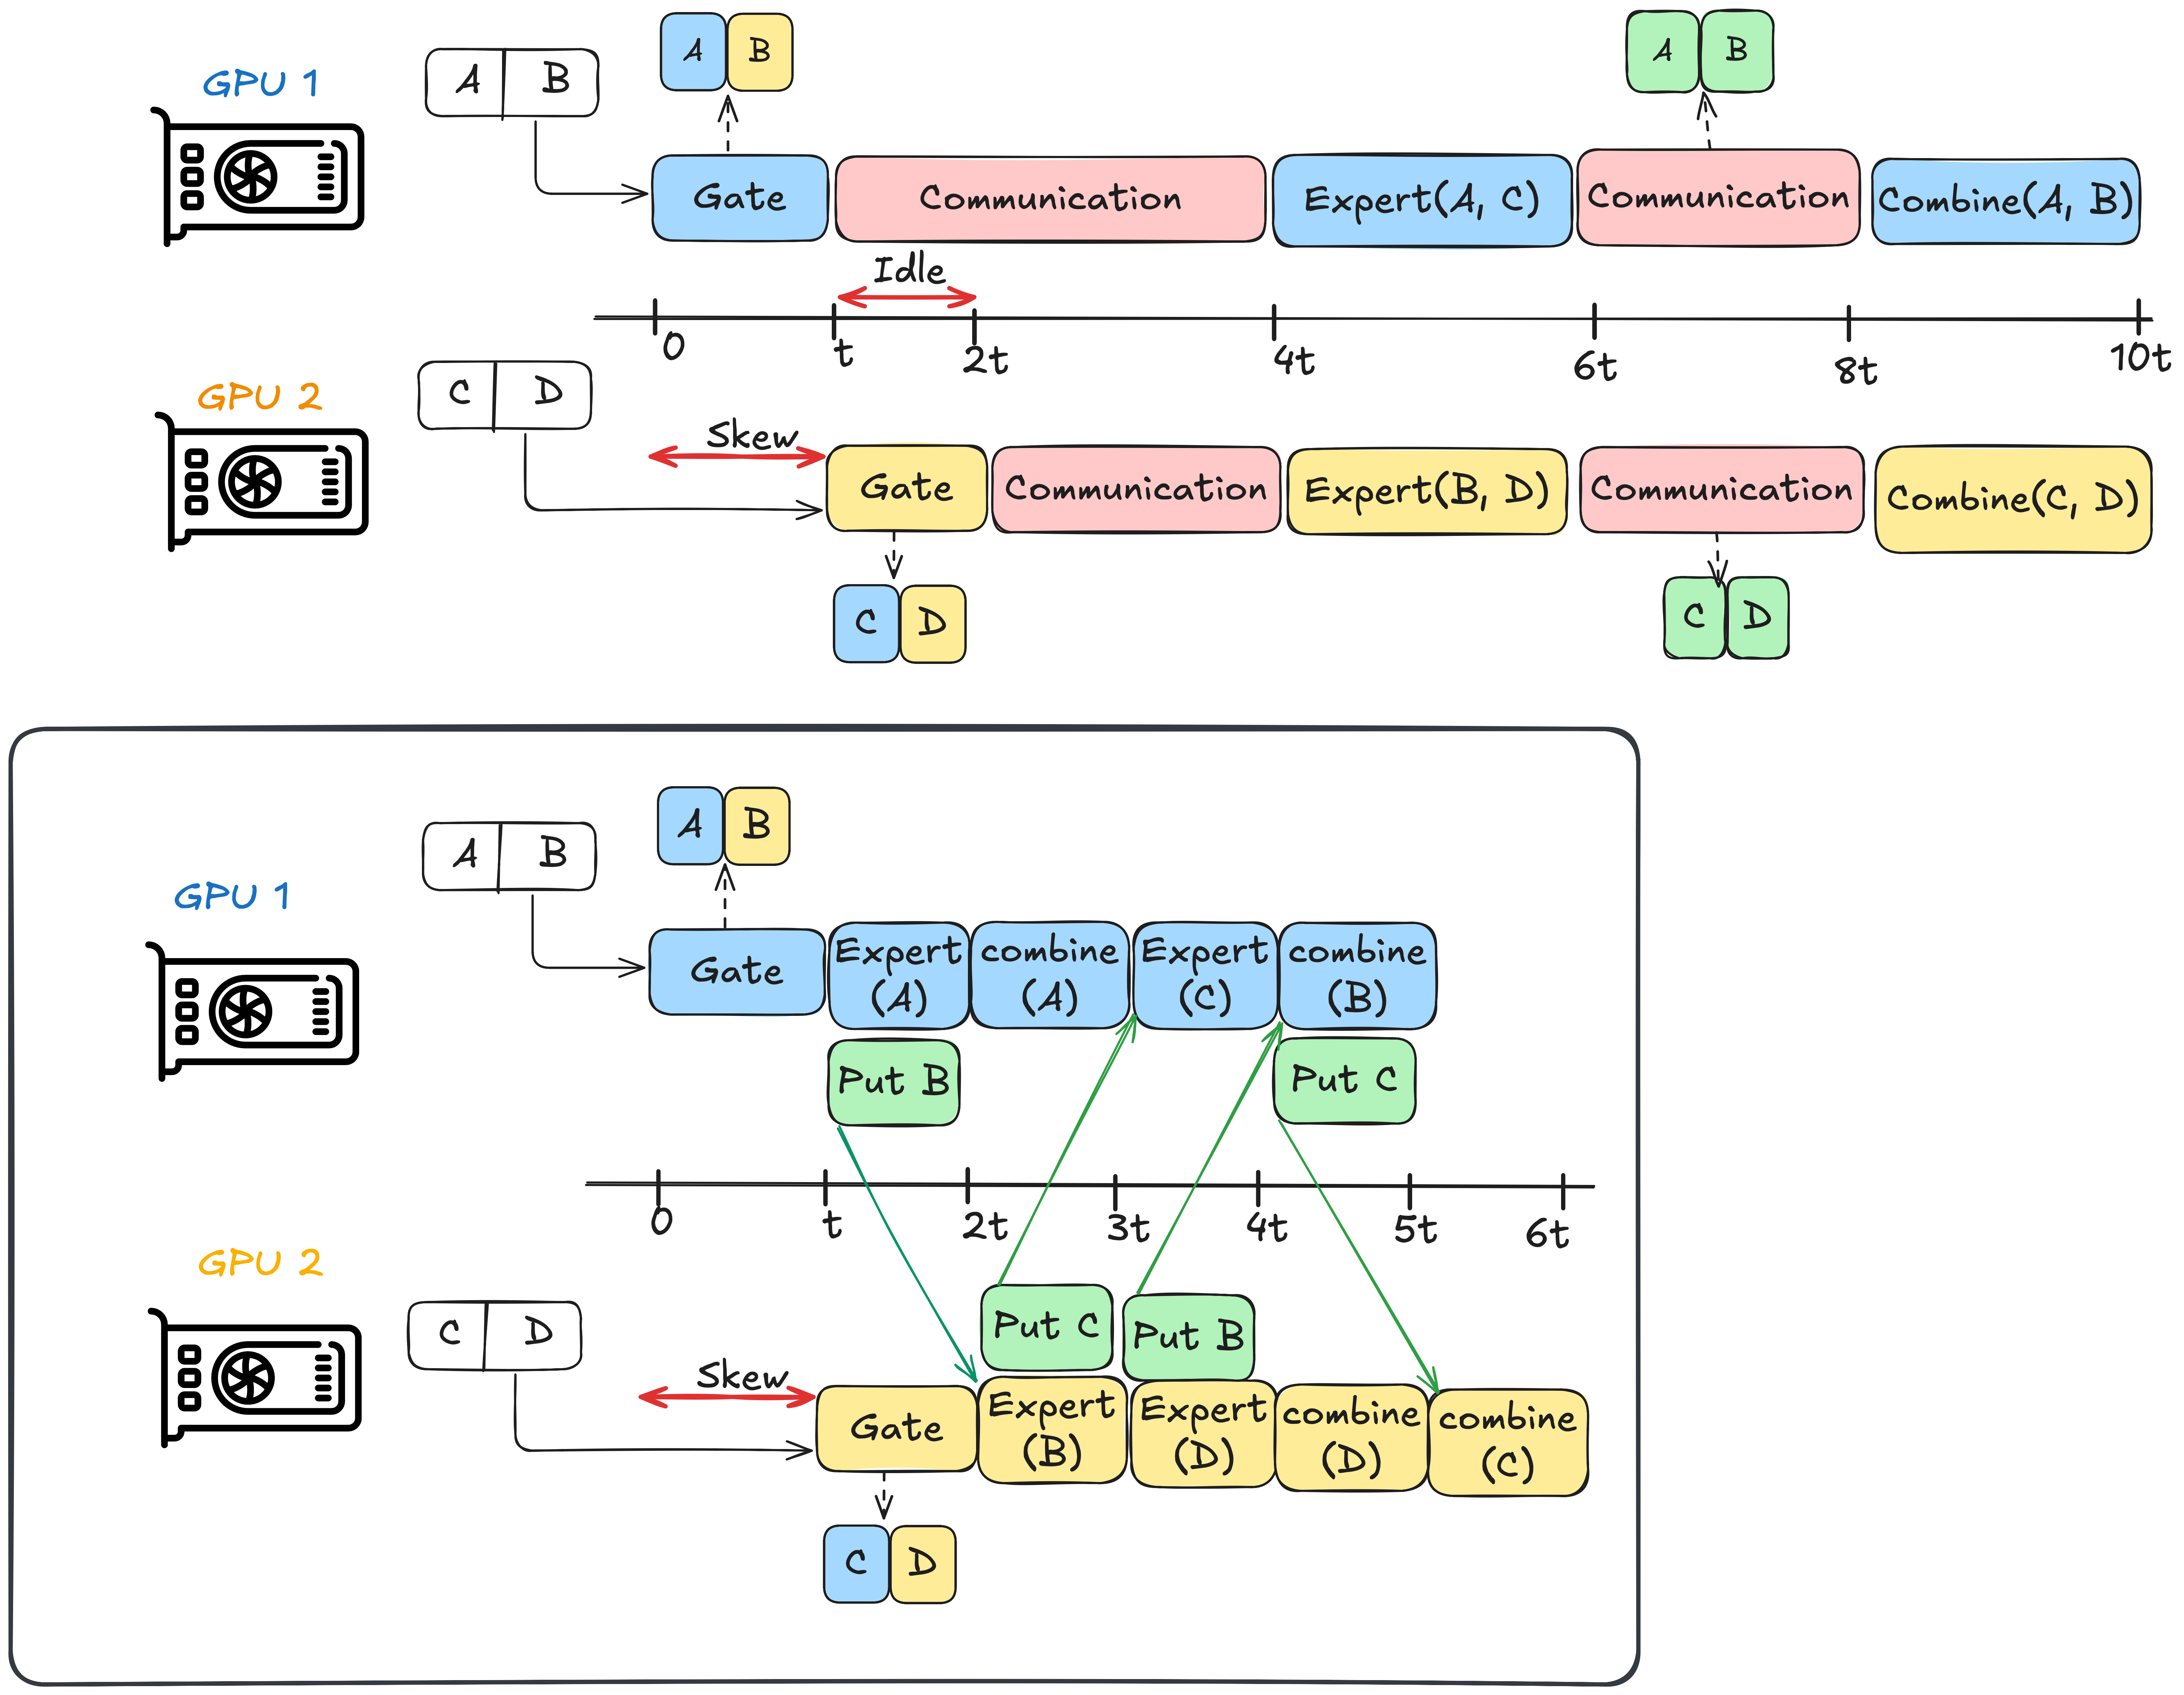
\includegraphics[width=0.98\textwidth, keepaspectratio]{figures/s_overlap}
    \caption{Overlapped Schedule (bottom) showing how idle time from the sequential schedule (top)
        is repurposed for computation. \sysname implements the overlapped schedule.}
    \label{fig:overlap}
\end{figure}
\alltoall communication as currently used in MoE frameworks is a ~\emph{synchronous} collective operation among
all participating GPUs. In this setting, disparities in processing speeds or kernel scheduling
among workers induce a straggler effect detrimental to the collective operation's performance.
Specifically, as shown in Figure~\ref{fig:straggler}, for distributed training of a 1.3B MoE model across 32 A100 GPUs,
we see P95 communication performance degradation of \textbf{1.32X} when compared to the mean actual kernel time
from Figure~\ref{sub:raw_perl}.
This performance reduction is rather tame as the underlying hardware is a supercomputer that is
well-tuned against ``software jitter''~\cite{nerscNetworkNERSC}.
On the other hand, the performance loss is more severe in a single node commodity Virtual Machine (VM) of
8 V100 GPUs with higher bandwidth, where we observe p95 performance reduction of \textbf{11X}.
In line with prior work~\cite{1639320, 10.1145/3545008.3545056} from the HPC community,
we argue that obviating the inherent barrier in this synchronous collective communication would
allow GPUs to repurpose this observed idle time for useful computation.
\section{Kernel Launch Overheads}\label{sec:kernel-launch-overheads}
\begin{figure}[!ht]
    \centering
    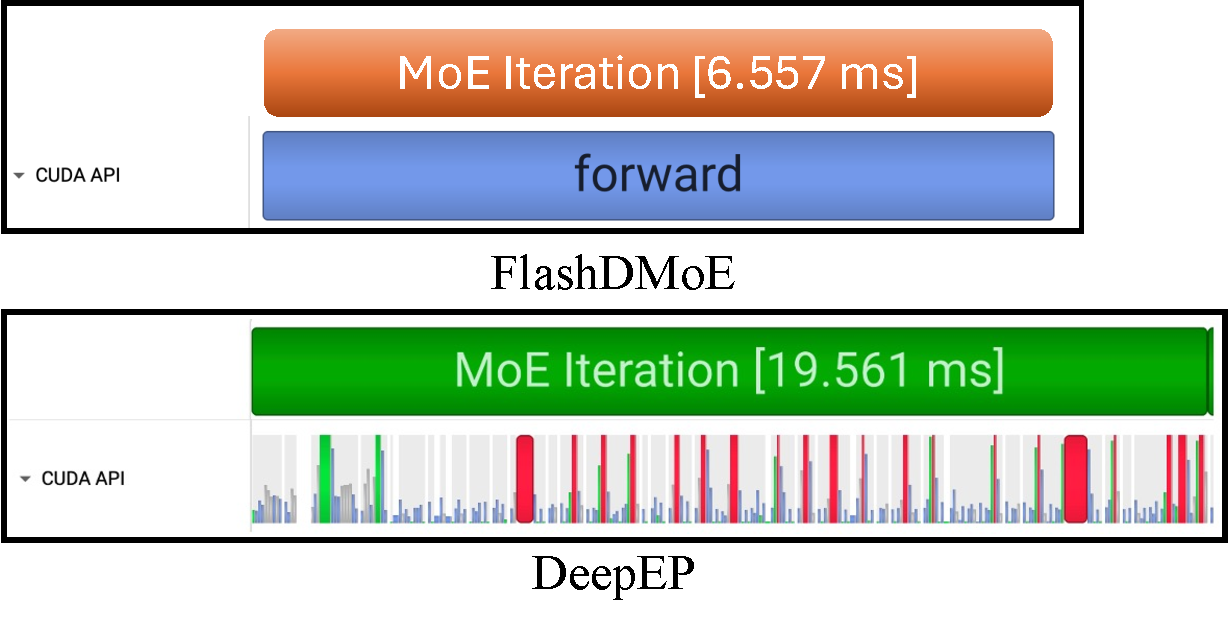
\includegraphics[width=0.8\textwidth, keepaspectratio]{figures/kernel_launch}
    \caption{Kernel Launch overhead (CUDA API row) juxtaposed with runtime latency.
    Compared to DeepEP that launches 432 kernels, \sysname launches a single one.}
    \label{fig:kl}
\end{figure}
We compare the kernel launch overheads between \sysname and existing baselines.
Table~\ref{tab:gpuOps} shows the number of kernel launches during a single forward pass: 
\sysname launches exactly one persistent kernel, 
while the baselines require up to 550 short-lived kernels.
Figure~\ref{fig:kl} visually compares \sysname and DeepEP~\cite{deepep} using CUDA API
traces captured by NSight Systems.
DeepEP exhibits numerous small CUDA API calls, while \sysname maintains high GPU
utilization by avoiding launch overhead and
synchronization gaps—achieving 93.17\% GPU utilization (\S\ref{ch:evaluation}) compared to 20.61\% for DeepEP.
%! Author = jonathan
%! Date = 5/27/25
\chapter{Method}\label{ch:method}
\begin{figure}[!ht]
    \centering
    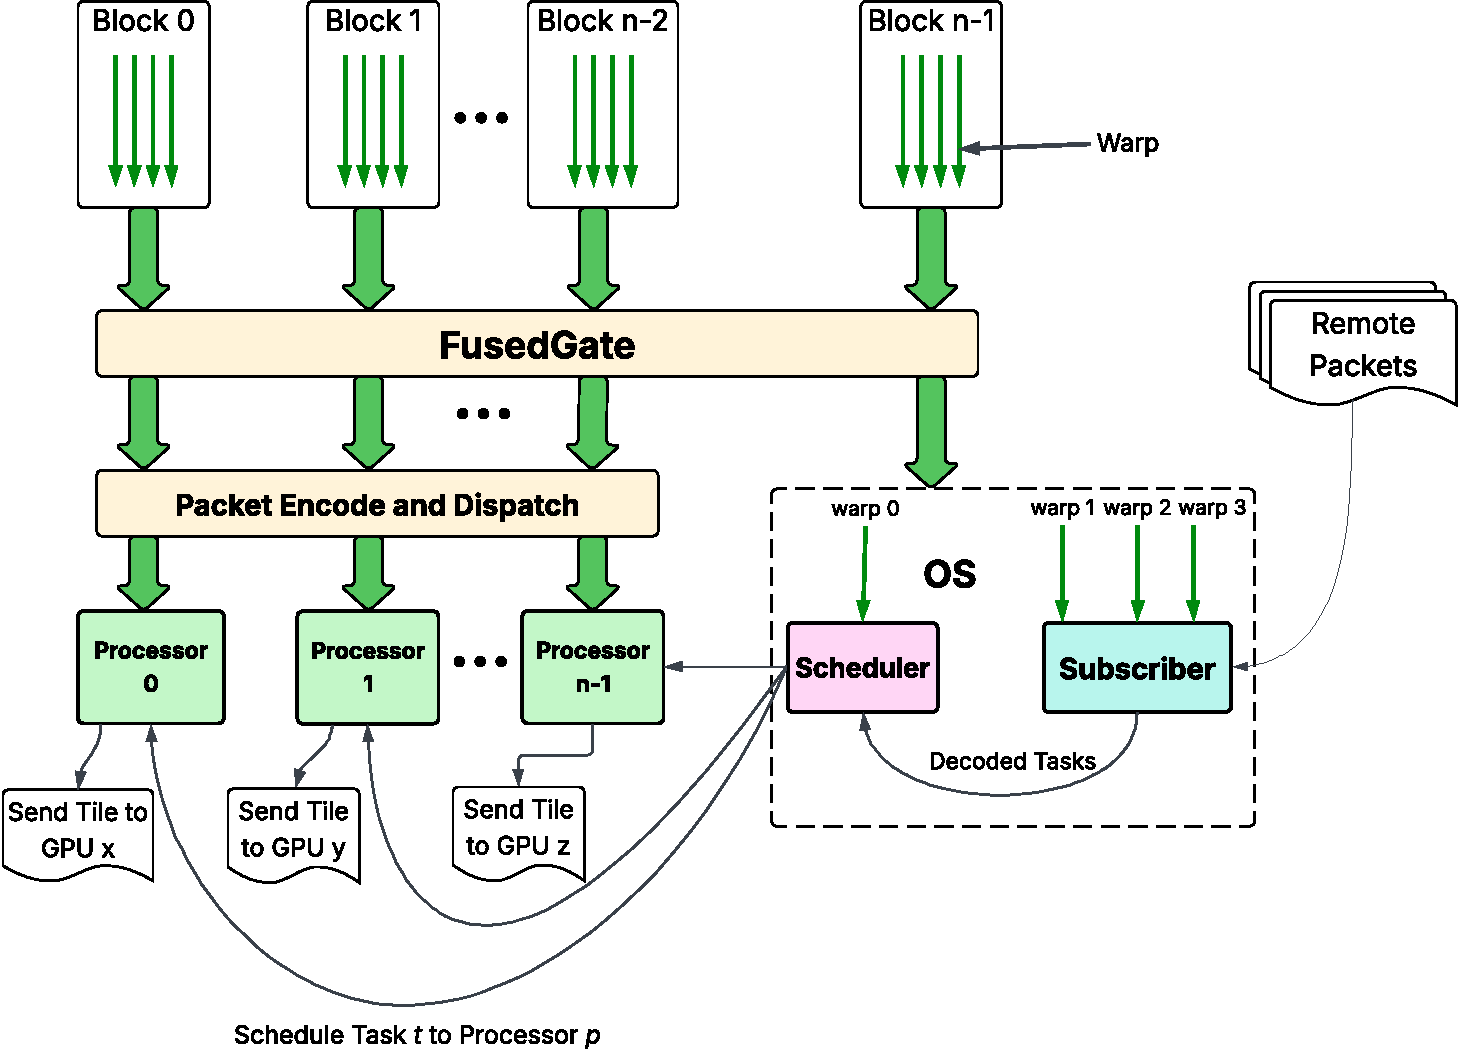
\includegraphics[width=0.8\textwidth, keepaspectratio]{figures/architecture}
    \caption{\emph{\sysname Fused Kernel}. Green arrows demonstrate block or warp specialization.}
    \label{fig:fusedK}
\end{figure}
The performance of modern distributed MoE systems suffers from two primary bottlenecks:
(1) frequent \alltoall collective communication operations on the critical execution path due to expert parallelism,
and (2) significant overhead from repeatedly launching multiple computation and communication kernels on the host CPU.
To overcome these limitations, we introduce \sysname, a fully fused MoE operator implemented as a single persistent GPU kernel.
Unlike previous approaches~\cite{comet, deepep, pmlr-v162-rajbhandari22a, megatron, MLSYS2023_5616d34c,
    MLSYS2024_339caf45, 10.1145/3503221.3508418, 10.1145/3588964, 10.1145/3627703.3650083,
    10.1145/3710848.3710868, NEURIPS2022_67d57c32}, \sysname is the first solution to implement a
\emph{completely fused Distributed MoE kernel}, eliminating kernel launch overhead entirely by
requiring only a single kernel launch (see Table~\ref{tab:gpuOps}).

\SetKwInput{KwRequire}{Require}
\SetKwInput{KwResult}{Result}
\SetKwInput{KwInput}{Input}
\SetKw{kwAnd}{and}
\SetKw{kwOr}{or}
\SetKw{kwTrue}{True}
\SetKw{kwFalse}{False}
\SetKwBlock{DoParallel}{do in parallel}{end}
\begin{algorithm}[!h]
    \DontPrintSemicolon
    \caption{~\emph{\sysname Distributed MoE Fused Kernel}}\label{alg:one}
    \KwInput{$A, O \in \mathbb{R}^{S\times H},\; E \in \mathbb{R}^{L\times H \times P},\; N$}
    \Begin{
        $T, G_{\phi} \gets \mathbf{FusedGate}(A)$\;
        \eIf{blockId $ + 1 < N$}{
            $\mathbf{Dispatch}(T, A)$\;
            processor::start()\;
        }{
            \eIf{$warpID == 0$}{
                scheduler::start()\;
            }{
                subscriber::start($E$, $O$)\;
            }
        }
    }
\end{algorithm}
\section{Actor Model}\label{sec:actor-model}
The design of \sysname is based on the actor model of concurrent
computation~\cite{agha:85, 10.5555/1624775.1624804, Greif:75}.
We implement this model by specializing GPU thread blocks and warps into three distinct actor roles:
(1) \textbf{Processor} (\S\ref{alg:processor}),
(2) \textbf{Subscriber} (\S\ref{alg:susbcriber}),
and (3) \textbf{Scheduler}(\S\ref{alg:scheduler}).
The Processor performs compute (GEMMs and element-wise operations)
and tile communication.
We use CUTLASS~\cite{Thakkar_CUTLASS_2023} as the underlying infrastructure for high-performance
BLAS routines and NVSHMEM for kernel-initiated communication~\cite{nvshm}.
The Subscriber and Scheduler perform administrative functions.
Specifically, the Scheduler assigns computational tasks to available thread blocks.
One key innovation is making the Scheduler both \emph{multithreaded},
enabling high scheduling throughput, and \emph{work-conserving},
ensuring consistently high GPU SM utilization.
On the other hand, the Subscriber subscribes to data communicated over the network.
Of the $N$ thread blocks on a GPU, we specialize $N-1$ to adopt the \textbf{Processor} role.
We specialize the last block for administrative functions.
Within this block, we specialize three warps for the \textbf{Subscriber} role and one warp
for the \textbf{Scheduler} role.
This split of thread blocks across actors is intentional:
our goal is to use few resources for administrative tasks while reserving
bulk of the resources for performing MoE computation tasks.
Figure~\ref{fig:fusedK} summarizes the \sysname architecture and its constituent actors,
while Algorithm~\ref{alg:one} gives a very close translation of the system in code.
\section{Inter-Actor Interactions}\label{sec:inter-actor-interactions}
\begin{figure}[!ht]
    \centering
    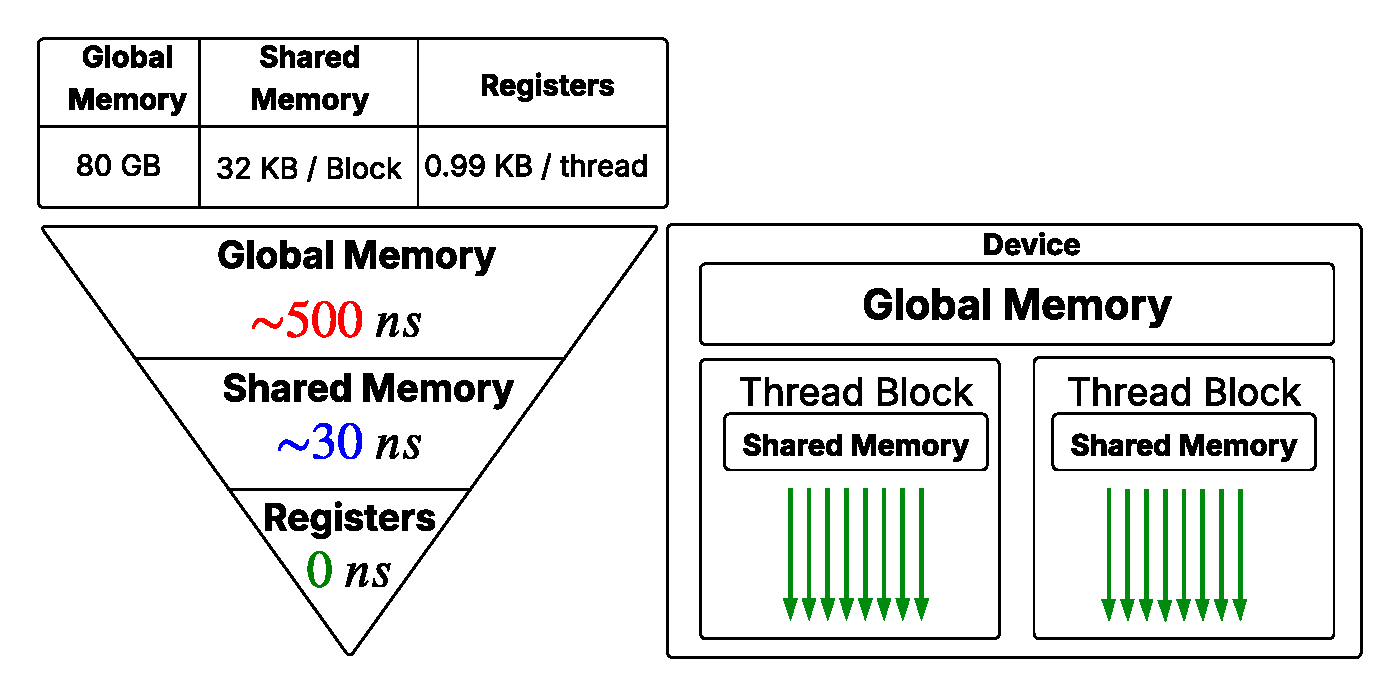
\includegraphics[width=4in, keepaspectratio]{figures/mem}
    \caption{\emph{GPU Memory Hierarchy}.
    The inverted pyramid (left) shows the load/store access latency~\cite{10579250, amperearch, ptx}. Table above outlines the capacity for different memory tiers (for A100 GPUs). The shared memory and register capacity are static configurations for \sysname.
    The right figure shows accessibility scopes: on-chip \textbf{registers}
    are scoped to a thread; on-chip \textbf{shared memory} is visible to all threads in a block;
    and off-chip \textbf{global memory} is accessible by all threads on device.}
    \label{fig:mem}
\end{figure}
\begin{figure}[!ht]
    \centering
    \vspace{-3mm}
    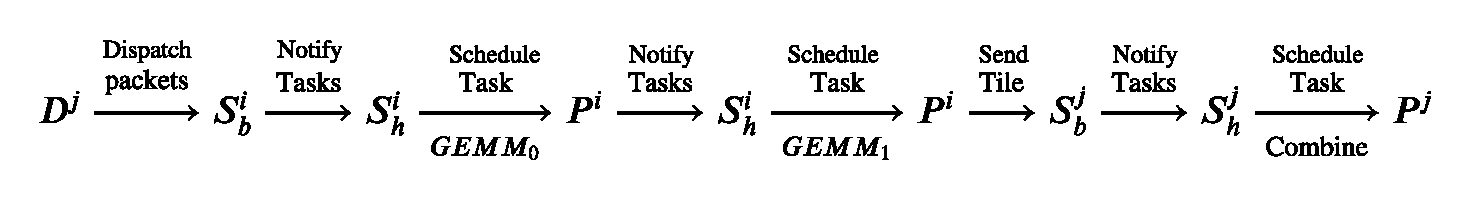
\includegraphics[width=\linewidth]{figures/actors}
    \caption{\emph{DMoE Functional Dependencies Expressed as a Chain of Actor Interactions}.
    We denote $S_b$, $S_h$, and $P$ as the
    Subscriber, Scheduler and Processor actors, respectively. For any actor $a \in \{S_b,\>S_b,\>P\}$,
        $a^i$ identifies an actor on GPU $i$. We define $D^j_i$ as the operator,
        where GPU $j$ dispatches packets of tiles to GPU $i$,
        This diagram expresses task dependencies at the granularity of a tile, namely
        $GEMM_0$, $GEMM_1$, combine and communication produce an output tile.
    }
    \label{fig:actors}
    \vspace{-4mm}
\end{figure}
\sysname decomposes MoE computation and communication at the granularity of a tile,
a statically sized partition of a tensor,
to achieve parallel execution and efficient overlap of tasks.
Each tile corresponds to a discrete unit of work encapsulated by a
\emph{task descriptor}.
The \textbf{Subscriber} actor decodes these
task descriptors from the remote data packets it receives.
Concurrently, the \textbf{Scheduler} actor receives notifications about
available tasks and batches them for execution by the \textbf{Processor} actors.
\textbf{Processor} actors perform computations defined by the tasks,
like the feed-forward network (FFN) and expert-combine operations.
Figure~\ref{fig:actors} shows the chain of actor interactions in \sysname
that comprise DMoE.
\begin{algorithm}[!ht]
    \DontPrintSemicolon
    \SetKwBlock{DoParallel}{do in parallel}{end}
    \caption{~\emph{Subscriber Actor}: executed by three warps}\label{alg:susbcriber}
    \Begin{
        $interrupt \gets \mathbf{GetSharedInterrupt}()$\;
        $flags \gets \mathbf{GetSymmetricFlags}()$\;
        $tQ \gets \mathbf{GetTQ}()$\;
        \tcp{Predefined upper bound on the number of tasks.}
        \tcp{Modulated to the actual task count computed}
        \tcp{from dispatch signals received from peer GPUs}
        $taskBound \gets \mathbf{GetTaskBound}()$\;
        \While{$\mathbf{AtomicLoad}(interrupt) == $ \kwFalse}{
            \tcp{dispatch flags}
            \DoParallel{
                Visit dispatch flags\;
                Atomically retrieve signal\;
                \If{Signal is set and flag is not visited}{
                    Mark visited\;
                    $\mathbf{SelfCorrectTaskBound}(taskBound, Signal)$\;
                    Enforce memory consistency before consuming packet\;
                    Decode packet into a set of $GEMM_0$ task descriptors\;
                    Write task descriptors to $tQ$\;
                    Notify Scheduler of decoded tasks\;
                }
            }
            Advance flags by number of dispatch flags length\;
            Atomically retrieve signal\;
            \tcp{combine signals}
            \DoParallel{
                Visit combine flags: one per tile\;
                \If{Signal is set and flag is not visited}{
                    Mark visited\;
                    Enforce memory consistency before consuming packet\;
                    Decode packet into a set of $combine$ task descriptors\;
                    Write task descriptors to $tQ$\;
                    Notify Scheduler of decoded tasks\;
                }
            }
        }
    }
\end{algorithm}
\begin{algorithm}[!ht]
    \DontPrintSemicolon
    \SetKwInput{KwInput}{Input}
    \SetKwBlock{DoParallel}{do in parallel}{end}
    \KwInput{$N$: Number of processors}
    \caption{~\emph{Scheduler Actor}: executed by one warp}\label{alg:scheduler}
    \Begin{
        $scheduled \gets 0$\;
        $tTB \gets 0$\;
        $tqS \gets \{\}$\;
        $pTDB \gets \mathbf{GetProcessorDoorbell}()$\;
        $sTDB \gets \mathbf{GetSubscriberDoorbell}()$\;
        $taskBound \gets \mathbf{GetTaskBound}()$\;
        $tTB \gets \mathbf{AtomicLoad}(taskBound)$\;
        \tcp{circular buffer ready queue}
        $rQ \gets \{\}$\;
        \tcp{Populate ready queue with Processor ids}
        $\mathbf{PopulateRQ}(rQ)$\;
        \While{$scheduled < tTB$}{
            $lt \gets 0$\;
            \DoParallel{
                Sweep doorbells and populate task counts into $tqS$\;
                Aggregate locally observed task counts into  $lt$\;
            }
            $qS,\>taskTally \gets 0$\;
            \tcp{qS is the inclusive output}
            $\mathbf{WarpInclusiveSum}(lt, qS, tasktally)$\;
            \While{$tasktally > 0$}{
                Repopulate $rQ$ with ready processor ids \;
                \DoParallel{
                    Starting at $rQ[qS]$ signal processors about tasks from $tqS$
                }
            }
            \If{$threadId == 0$}{
                $tTB \gets \mathbf{AtomicLoad}(taskBound)$\;
            }
            $tTB \gets \mathbf{WarpBroadcast}(tTB)$
        }
        $\mathbf{InterruptSubscribers}()$\;
        $\mathbf{InterruptProcessors}()$\;
    }
\end{algorithm}
\begin{algorithm}[!h]
    \DontPrintSemicolon
    \caption{~\emph{Processor Actor}: executed by a block}\label{alg:processor}
    \Begin{
        $tQ \gets \mathbf{GetTQ}()$\;
        $signal \gets 0$\;
        \tcp{shared memory variables}
        $task \gets \{\}$\;
        $interrupt \gets \kwFalse$\;
        $complete \gets \kwFalse$\;
        \While{$interrupt == $ \kwFalse}{
            \If{$warpId == 0$}{
                \If{$threadId == 0$}{
                    $\mathbf{awaitTaskFromScheduler}(interrupt,\>signal)$\;
                    $\mathbf{FencedNotifyRQ}(ready)$\;
                }
                $\mathbf{syncwarp}()$\;
                $\mathbf{warpReadTQ}(tQ, \>signal, \>task)$\;
            }
            $\mathbf{syncthreads}()$\;
            \If{$interrupt == $ \kwFalse}{
                \Switch{task.Type}{
                    \Case{$GEMM_0$}{
                        \tcp{fused GEMM, epilogue and async tile staging}
                        $\mathbf{fGET}(GEMM_0, \>task)$\;
                        \If{$threadId == 0$}{
                            $complete \gets \mathbf{NotifyTileCompletion}()$\;
                        }
                        $\mathbf{syncthreads}()$\;
                        \If{$complete == \kwTrue$}{
                            $\mathbf{NotifySchedulerNextGEMM}(tQ)$\;
                        }
                    }
                    \Case{$GEMM_1$}{
                        \tcp{fused GEMM, epilogue and async tile transfer}
                        $\mathbf{fGET}(GEMM_1, \>task)$\;
                    }
                    \Case{$Combine$}{
                        $\mathbf{combine}(task)$\;
                    }
                }
            }
        }
    }
\end{algorithm}
\section{Tiling}\label{sec:tiling}
Selecting appropriate tile dimensions in \sysname is crucial to ensure efficient GPU utilization.
A small-sized tile underutilizes the GPU's tensor cores,
while excessively large tiles create register pressure,
causing performance-degrading register spills to local memory.
After careful parameter sweeps,
we choose tile dimensions of (128, 64).
Our key insights are: increasing tile width raises the register usage per thread,
potentially triggering costly spills;
increasing tile height without adjusting thread count increases workload per thread, harming performance.
Raising the thread count per block beyond our fixed value of 128 threads reduces the number of concurrent blocks,
negatively affecting SM occupancy.
Larger thread-block sizes also increase overhead from intra-block synchronization (\emph{\_\_syncthreads()} barriers),
further degrading performance.
Thus, our chosen tile dimensions deftly balance these constraints.
%! Author = jonathan
%! Date = 5/27/25
\chapter{Programming Abstractions}\label{ch:abstraction}
\section{Task}\label{sec:task}
We describe the FFN in \S\ref{sec:comoutational-cost-equivalence}, so here we explicate the \emph{combine} operation.
The expert-combine operation, used in architectures like GShard~\cite{DBLP:conf/iclr/LepikhinLXCFHKS21}
and DeepSeek~\cite{deepep}, merges outputs from multiple experts by computing a weighted combination based
on their affinity scores:
\begin{equation}\label{eq:combine1}
\mathcal{C}_i = \sum\limits_{j = 1}^k g_{i, e}
\end{equation}
\begin{equation}\label{eq:combine2}
\mathbf{h}_i = \sum\limits_{j = 1}^k \frac{g_{i, e}}{\mathcal{C}_i}\cdot \mathbf{h}_i^k
\end{equation}
Above, $i \in {0, S - 1}$ represents an input token index, $e = E_{i,k}$ identifies the $k$-th expert
selected for token $i$, and $g_{i,e}$ is the affinity score indicating how relevant expert $e$ is for token $i$.
\section{Unified Abstraction}\label{sec:unified-abstraction}
We unify the FFN and combine operations under a common abstraction called a \emph{task}.
Tasks provide a uniform interface for communicating tile-level work among Subscribers, Schedulers, and Processors.
Formally, a task descriptor $t \in \mathcal{T}$ is defined as a tuple:
\[
    t = (\mathcal{M}, \star, \phi)
\]
where $\mathcal{M}$ is a set of metadata (such as device ID, tile index), $\star$ is a binary tensor operation
(specifically, matrix multiplication $\cdot$ or Hadamard product $\odot$), and $\phi$ is an element-wise activation
function (e.g., ReLU or identity).
We define a task $t$ operating on input tensors $A$, $B$, $D$, producing output tensor $C$, as follows:
\begin{equation}\label{eq:task_def}
\mathcal{F}_t(A, B, C, D) \coloneqq C \gets \phi\left(A \star_t B + D\right)
\end{equation}

The operator $\star_t$ (instantiated from $\star$) may behave differently depending on the task metadata $\mathcal{M}$,
and the result of $A \star_t B$ is accumulated into $D$.
We provide an example of task metadata in Figure \ref{fig:task}.
\begin{figure}[!ht]
    \centering
    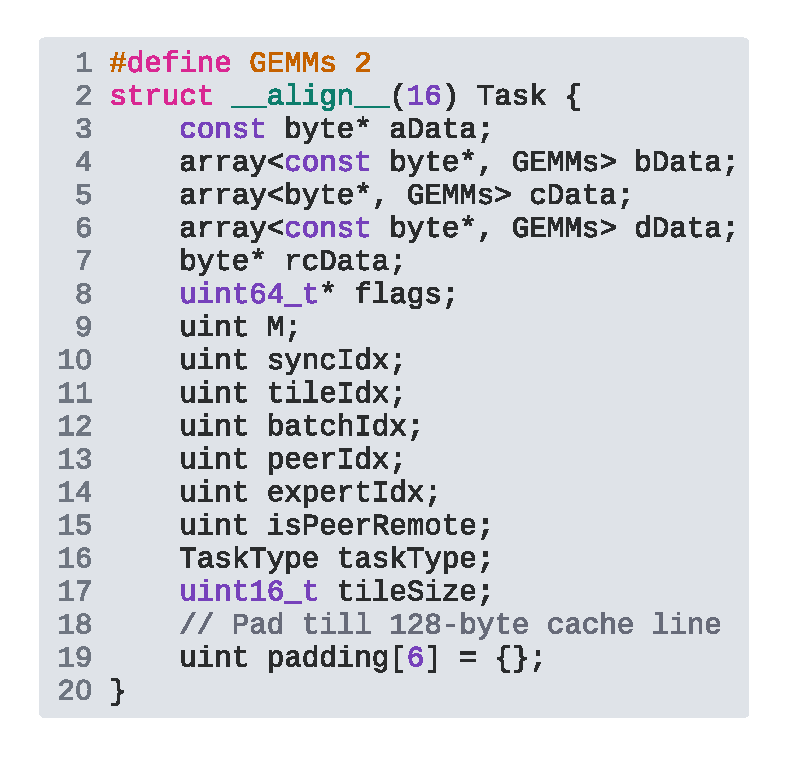
\includegraphics[width=4in]{figures/task}
    \caption{\emph{Task Struct}. $\text{TaskType} \in \{GEMM_0,\>GEMM_1,\>Combine\}$}
    \label{fig:task}
\end{figure}

In practice, we implement each task defined by Equation~\ref{eq:task_def} as a \emph{single fused} \verb|__device__|
decorated function which the \textbf{Processor} (Algorithm \ref{alg:processor}) invokes at runtime.
Fusion for $t$ entails applying $\phi$ and the succeeding addition operation to registers
storing the results of the binary operator $\star_t$.
To illustrate its flexibility, we show how the FFN and expert-combine operations can be expressed
using this task framework.
Note that we omit the matrix multiplication symbol ($\cdot$) for simplicity.
Also, $\phi_1$ can be any activation function, while $\phi_2$ is the identity function.
The FFN is expressed as:
\begin{gather*}
    t_1 = (\mathcal{M}, \cdot, \phi_1), \quad t_2 = (\mathcal{M}, \cdot, \phi_2), \\
    \mathcal{F}_{t_1}(A, B_1, C_1, D_1) \coloneqq C_1 \gets \phi_1\left(A B_1 + D_1\right), \\
    \mathcal{F}_{t_2}(C_1, B_2, C_2, D_2) \coloneqq C_2 \gets \phi_2\left(C_1 B_2 + D_2\right).
\end{gather*}
Whereas, the expert-combine operation is formalized as:
\begin{gather*}
    t_3 = (\mathcal{M}, \odot, \phi_2), \\
    \mathcal{F}_{t_3}(A, S, C, C) \coloneqq C \gets \phi_2\left(A \odot S + C\right).
\end{gather*}
\section{Symmetric Tensor Layout for Inter-GPU Communication}\label{sec:symmetric-tensor-layout}
\begin{figure}[!ht]
    \centering
    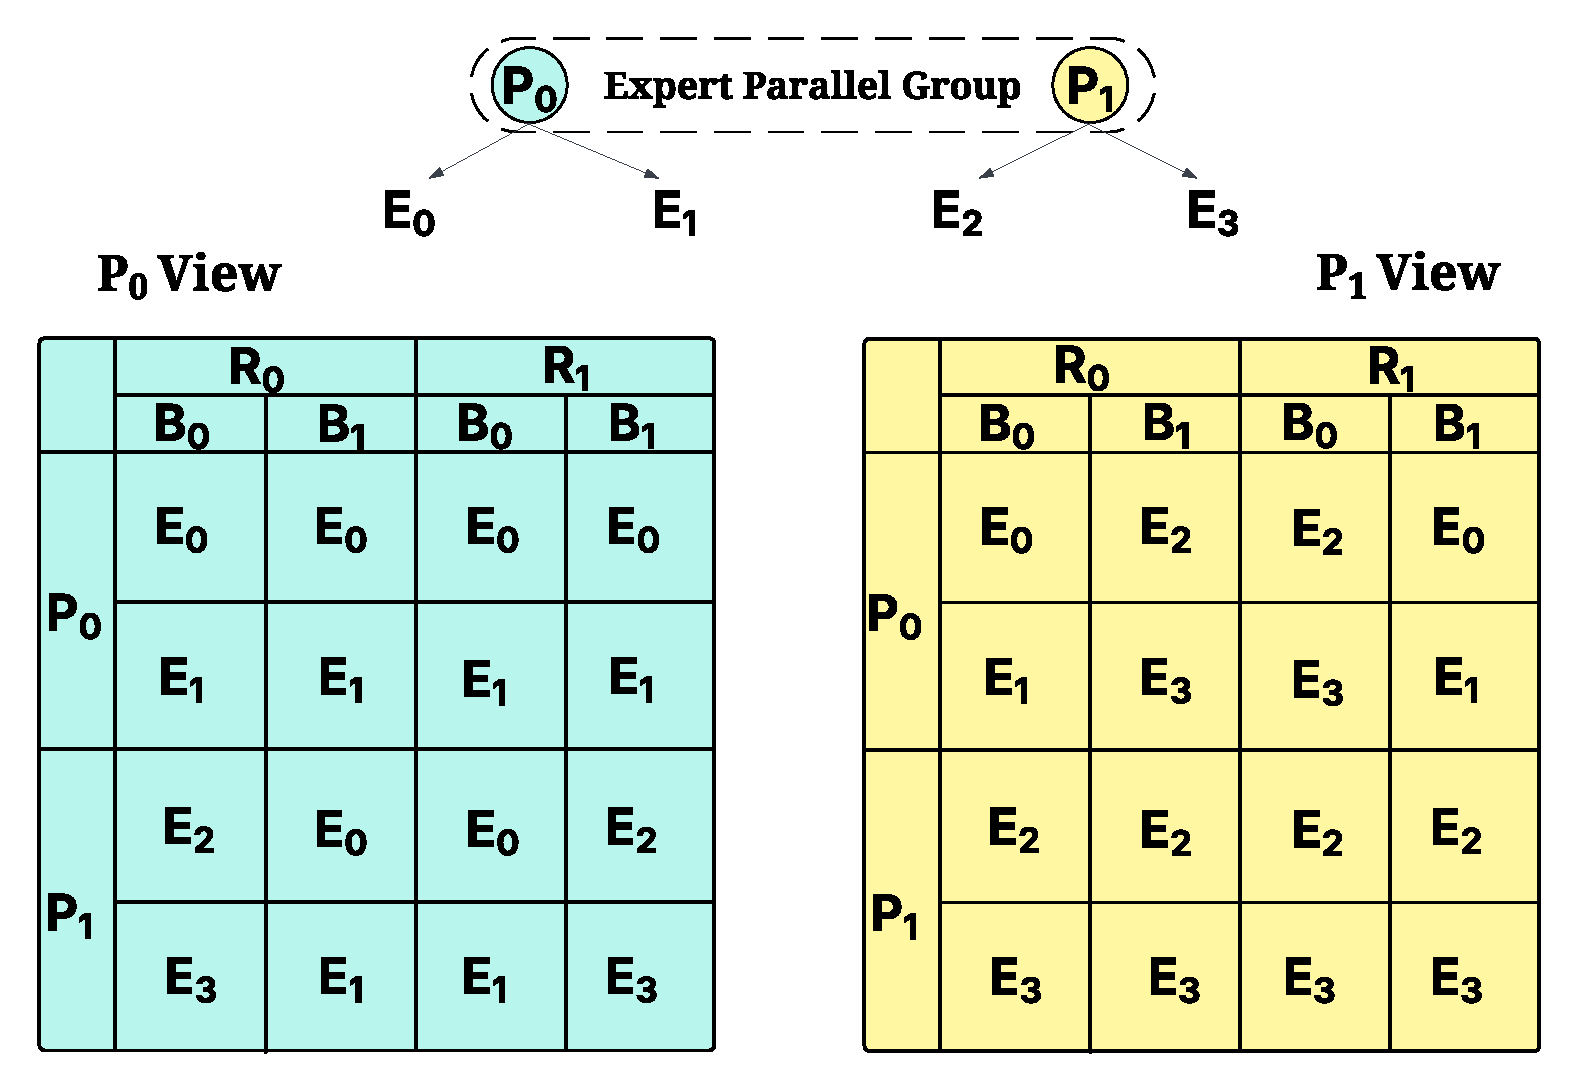
\includegraphics[width=0.85\linewidth, keepaspectratio]{figures/mem_layout}
    \caption{\emph{Symmetric Tensor Layout across 2 Expert-parallel Processes}.}
    \label{fig:mem_layout}
\end{figure}
Within a single GPU device, the actors in \sysname communicate through the GPU's memory subsystem (see Figure~\ref{fig:mem}).
Specifically, the Scheduler and Subscriber actors exchange data via fast shared memory, while other actor
pairs communicate through global memory.
For communication across multiple devices, \sysname uses \emph{device-initiated communication},
leveraging the one-sided PGAS (Partitioned Global Address Space) programming model~\cite{10.1145/1278177.1278183}.
However, achieving scalable and correct one-sided memory accesses in PGAS without costly synchronization
is a known challenge~\cite{deepep, triton-dist}.
We address this challenge with a provably correct and scalable solution: a symmetric tensor layout $L$,
supporting fully non-blocking memory accesses.
We define L as:\\
\[
    L \in \mathbb{R}^{P\times R \times B \times E \times C \times H}
\]
where: $P$ is the expert parallel world size, $R$ identifies communication rounds
(two rounds, one for token dispatch and one for combine), $B$ is number of staging buffers,
$E$ is the number of local experts, $C$ is the upscaled expert capacity (\S\ref{sec:payload})
and $H$ is the embedding dimension.
\begin{figure}[!ht]
    \centering
    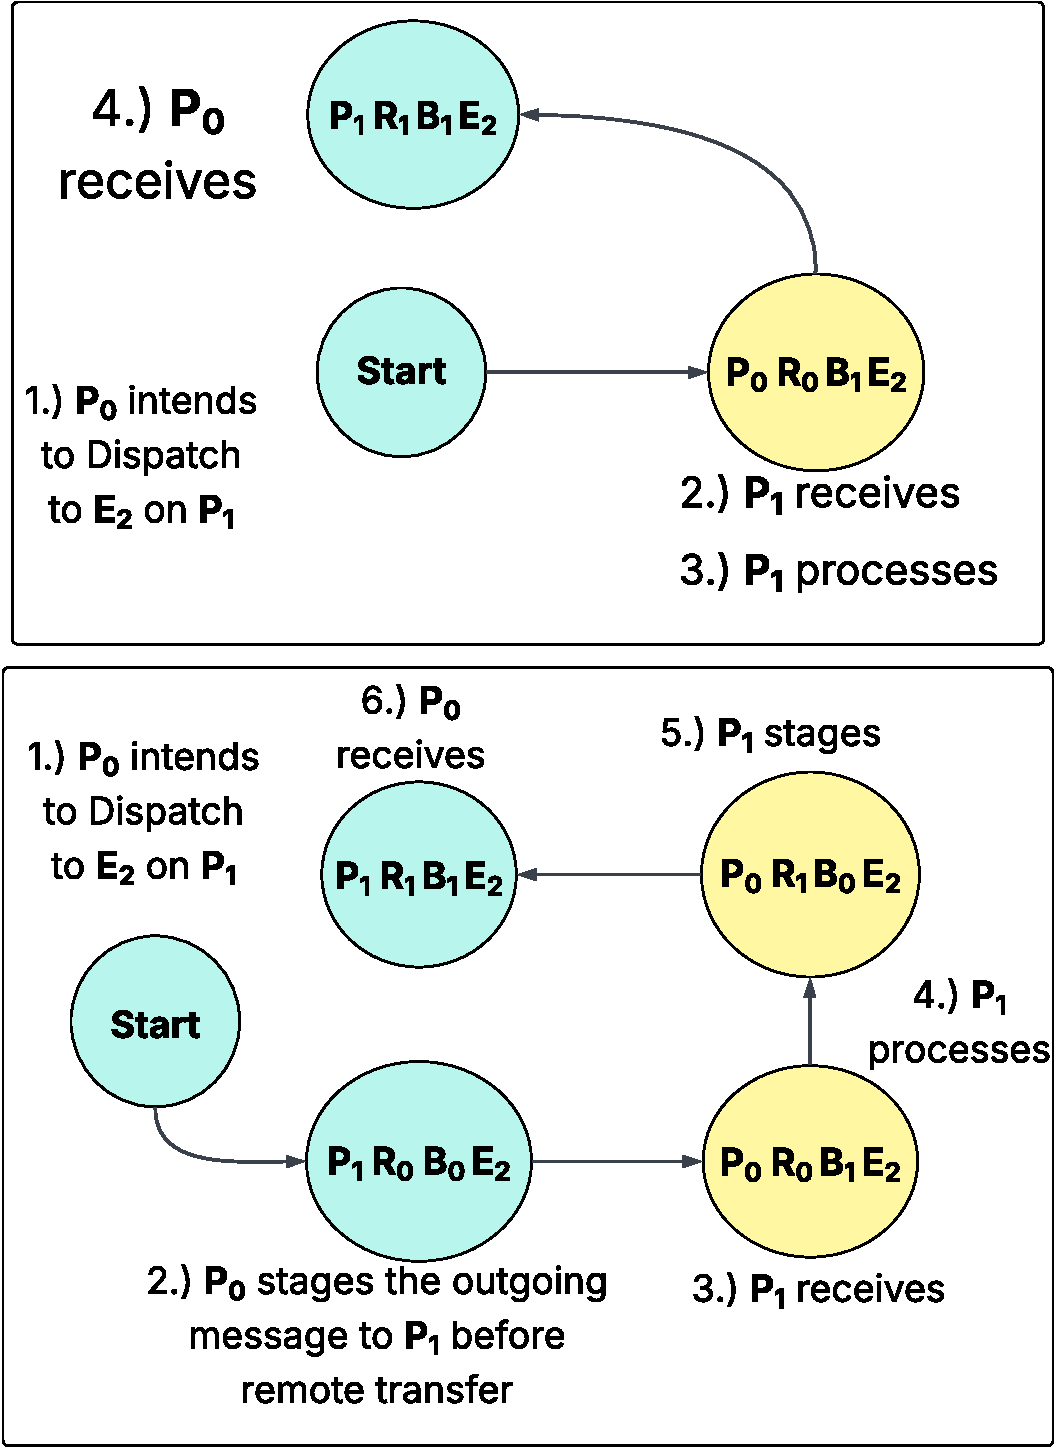
\includegraphics[width=0.7\textwidth, keepaspectratio]{figures/sm_big}
    \caption{\emph{State machine for DMA (top) and RDMA (bottom) communication.}}
    \label{fig:sm}
\end{figure}
Our core insight to enable non-blocking communication is \emph{temporal buffering}.
Specifically, we overprovision memory for the underlying token matrix by at least $2 \cdot r$ times, where $r$ is the number of communication rounds in the dependency graph, and the factor of $2$ accounts for separate buffers for incoming and outgoing data within each communication round. For MoE models, we have $2 \cdot r = 4$.
This modest increase in memory usage eliminates the need for synchronization during one-sided data transfers.
Figure~\ref{fig:sm} illustrates how cells within this symmetric tensor layout are indexed
and used for Direct Memory Access (DMA) and Remote DMA (RDMA) operations.
As Theorem~\ref{theorem:ww} reinforces,
this indexing scheme over $L$ is the underlying mechanism that allows for fully non-blocking accesses eliding
synchronization because all accesses are write \emph{conflict-free}.
\begin{definition}
    Define a write as~$w(p_s, p_t, i)$, where $p_s$ is the source process and $i$ is an ordered tuple
    indicating the index coordinates for $L$ residing on the target process $p_t$.
    A write-write conflict occurs when there exist at least two distinct, un-synchronized, concurrent writes
    $w_1(p_{s_1}, p_{t_1}, i_1)$ and $w_2(p_{s_2}, p_{t_2}, i_2)$, such that
    $p_{t_1} = p_{t_2}$ and index coordinates $i_1 = i_2$ but $p_{s_1} \neq p_{s_2}$
\end{definition}
\begin{definition}
    For any source process $p_s$, a valid index coordinate $i = (p*, r, b, e, c)$ satisfies the following:
    \begin{enumerate}
        \item For inter-device writes, it must hold that $p* = p_s$ and $b = 1$.
        Note this also applies to self-looping writes $w(p_t, p_t, i)$.
        \item For any write $w(p_s, p_t, i)$, if $b = 0$, then $p_s = p_t$.
        This rule describes intra-device staging writes.
    \end{enumerate}
\end{definition}
\begin{theorem}\label{theorem:ww}
$L$ is write-write conflict-free.
\end{theorem}
\begin{proof}
    As is the case for typical physical implementations,
    assume that each index coordinate $i$ maps to a distinct memory segment in $L$.
    Next, we show by contradiction that no write-write conflicts can exist when accessing $L$ using \emph{valid} $i$.
    For simplicity, we only include the index coordinates when describing a write.
    Assume that there exist at least two writes $w_1(p_{s_1}, p_{t_1}, i_1),\>w_2(p_{s_2}, p_{t_2}, i_2)$
    with $p_{t_1} = p_{t_2}$ and valid destination coordinates
    $i_1, i_2$, where $i_1 = i_2$ lexicographically and both are unpacked below.
    \[
        i_1 = (p_1, r_1, b_1, e_1, c_1),\> i_1 = (p_2, r_2, b_2, e_2, c_2)
    \]
    Note that for the message staging state, even though $i_1 = i_2$ the resultant memory segments reside in
    different physical buffers resident in $p_{s_1}$ and $p_{s_2}$ respectively.
    Therefore, for this state, there are no conflicts as intra-process writes always have distinct $c_j$
    coordinates, where $j \in \{0, C - 1\}$.
    For inter-process transfers, we have two cases.

    \textit{Case 1: $p_{s_1} = p_{s_2}$}
    \newline Here, $w_1$ and $w_2$ are identical operations.
    This contradicts the definition of a conflict, which requires that $p_{s_1} \neq p_{s_2}$.
    In practice, such repeat writes never even occur.

    \textit{Case 2: $p_{s_1} \neq p_{s_2}$}
    \newline To ensure validity for $i_1$ and $i_2$, it is the case that $p_1 = p_{s_1}$ and $p_2 = p_{s_2}$.
    However, this implies that $i_1 \neq i_2$ yielding a contradiction as desired.
\end{proof}
To construct $L$, we start from the original token buffer $T \in \mathbb{R}^{S \times H}$, where $S$ is the sequence length and $H$ is the hidden dimension. We first reorganize the sequence dimension $S$ into three sub-dimensions representing the expert capacity ($C$), local expert slots ($E$), and the expert parallel world size ($W$), st:
\[
    C \cdot E \cdot W = C \cdot E' = S', \quad\text{where}\quad S' \geq S \text{ and } E' \geq E_W
\]
In the typical case of uniform expert distribution (illustrated in Figure~\ref{fig:mem_layout}),
we have $S' = S$ and $E' = E_W$, where $E_W$ is the total number of experts in the model.
Thus, the size of the token buffer is $Size(T) = S' \cdot H$.
In Figure~\ref{fig:mem_layout}, each cell labeled $E_i$ (with $i \in \{0,\ldots,3\}$) is a matrix of size $(C, H)$.
Extending prior work~\cite{DBLP:conf/iclr/LepikhinLXCFHKS21, comet}, we introduce additional temporal dimensions $R$
(communication rounds) and $B$ (staging buffers).
Each communication round has two fixed staging slots:
one for outgoing tokens and another for incoming tokens.
Each slot, indexed by dimension $P$, forms a tensor of shape $(S', H)$.
Therefore, the tensor size $Size(L)$ is generally at least four times the original token buffer size,
becoming exactly four times larger in the case of uniform expert distribution.
Empirically (\S\ref{sec:eval:memory}), we find:
\[
    Size(L) \approx 4 \cdot Size(T)
\]
\section{In-place Padding for Payload Efficiency}\label{sec:payload}
Due to the dynamic and uneven distribution of tokens in MoE dispatch~\cite{bmamba},
GPUs commonly receive fewer tokens than their predefined expert capacity.
Current MoE frameworks~\cite{pmlr-v162-rajbhandari22a}
typically pad these buffers with null tokens before computation,
unnecessarily increasing communication payloads and degrading performance.
In contrast, we propose \emph{in-place padding},
performing padding directly within the local symmetric tensor buffers and
thus eliminating excess network communication.
As we show in Figure~\ref{fig:mem_layout} as a reference,
each cell $E_i$ is sized according to the expert capacity $C$.
We further align this capacity to ensure divisibility by the tile block size $bM = 128$,
guaranteeing safe and aligned memory reads by Processor threads consuming remote tokens.
This in-place padding strategy slightly increases the memory footprint of $L$, as described below:
\[
    Size(L) \approx \begin{cases}
                        4 \cdot Size(T), & \frac{S}{E} \geq bM \\[1ex]
                        4 \cdot \frac{bM \cdot E}{S} \cdot Size(T), & \text{otherwise}
    \end{cases}
\]
%! Author = jonathan
%! Date = 5/27/25
\chapter{Evaluation}\label{ch:evaluation}
\begin{table}[h]
    \centering
    \caption{Implementation metrics of~\sysname using fully inlined NVSHMEM.}
    \label{tab:impl_metrics}
    \begin{tabular}{cc}
        \toprule
        \textbf{Metric} & \textbf{Value}\\ \hline
        Total lines of code (CUDA/C++) & 6820 \\
        Kernel stack frame size & 0 B \\
        Spill stores (per thread) & 0 \\
        Spill loads (per thread) & 0 \\
        Shared memory usage (per block) & 46 KB \\
        Registers per thread & 255 \\
        Max active blocks per SM & 2 \\
        Compilation time & 53 seconds \\
        Binary size & 29 MB\\
    \end{tabular}
\end{table}
We implement (Table~\ref{tab:impl_metrics}) and evaluate \sysname by addressing two main questions:
(1) Under what conditions does \sysname outperform state-of-the-art MoE systems,
and why (\S\ref{subsec:scalability-with-tokens-and-experts} -~\ref{sec:payload-efficiency})? and (2) How much GPU memory does
\sysname require for core data structures (\S\ref{sec:eval:memory})?
\section{Setup}\label{sec:setup}
We run experiments on a RunPod server with 8 $\times$ NVIDIA H100 80G GPUs, 125 GB of RAM, and 20 vCPUs.
We used PyTorch 2.6.0, CUDA 12.8, and Ubuntu 22.04.
All experiments use MoE transformer models configured with 16 attention heads,
an embedding dimension of 1024, and an FFN hidden size of 4096.
We use top-2 routing with a capacity factor of 1.0.
Note all baselines were evaluated using FP16 precision, while \sysname was evaluated on FP32 precision,
see \S\ref{ch:limitations-and-future-work} for more details.
We compare \sysname against several state-of-the-art MoE systems:
(1) \textbf{Comet}~\cite{comet},
(2) \textbf{FasterMoE}~\cite{fastermoe},
(3) \textbf{Megatron-LM}~\cite{megatron-lm}, and
(4) \textbf{DeepEP}~\cite{deepep}.
Comet and DeepEP rely on NVSHMEM for communication, while FasterMoE and Megatron-LM use NCCL.
We also evaluate \sysname on a multi-node environment and discuss our findings in \S\ref{sec:multi-node-evaluation}.
\section{Scalability with Tokens and Experts}\label{subsec:scalability-with-tokens-and-experts}
\begin{figure}[h!]
    \centering
    \subcaptionbox{Scaling with the number of tokens (E = 32).\label{fig:scalability-token}}{%
        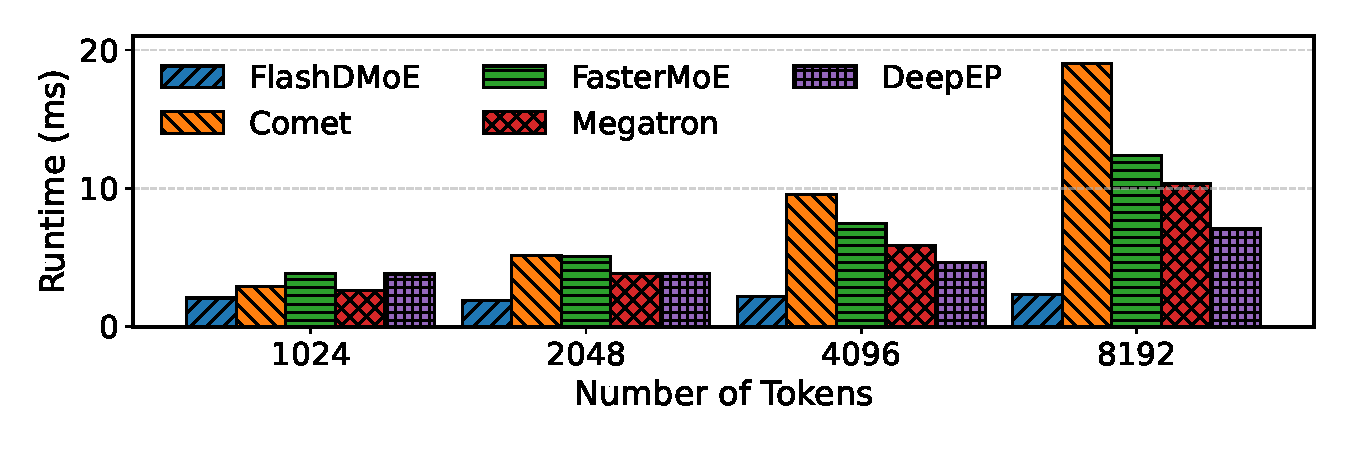
\includegraphics[width=\linewidth]{figures/scaling_tokens}
    }
    \subcaptionbox{Scaling with the number of experts (T = 8K)\label{fig:scalability-experts}}{%
        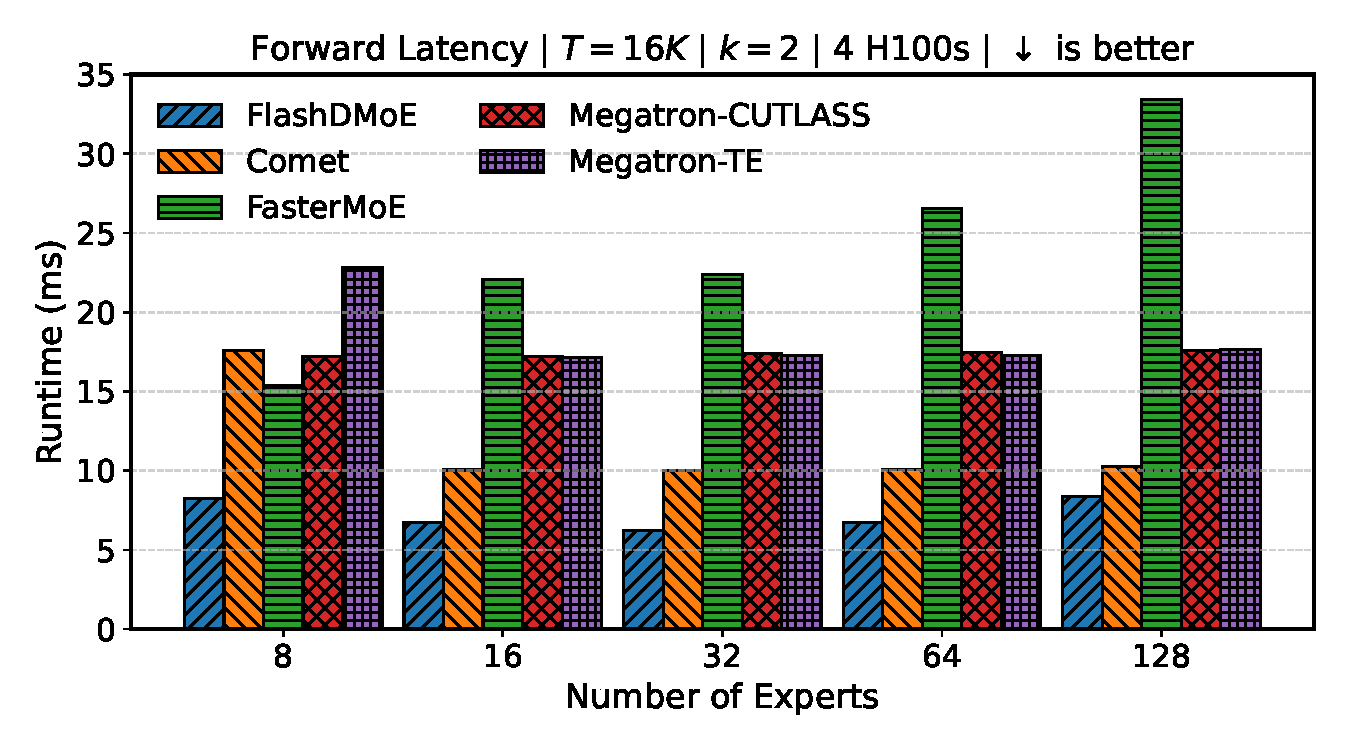
\includegraphics[width=\linewidth]{figures/scaling_experts}
    }
    \caption{Scalability with respect to the number of tokens and experts. All experiments use 8 GPUs.}
    \label{fig:scalability-token-experts}
\end{figure}
We first analyze the scalability of \sysname in two dimensions: the number of input tokens and the number of experts.
Figure~\ref{fig:scalability-token-experts} shows execution time for a single MoE layer on 8 GPUs.
\sysname outperforms baselines between \textbf{1.4X} to \textbf{9.5X} when scaling across sequence lengths and
between \textbf{1.2X} to \textbf{15X} across number of experts.
We provide raw performance numbers in \S\ref{sec:numerical-data}.

When scaling number of tokens (Fig.~\ref{fig:scalability-token}),
\sysname maintains near-constant execution time ($2.07-2.33$ ms).
In contrast, baselines incur significant runtime increases.
For example, Comet's runtime grows from 2.9 ms to 19 ms,
FasterMoE from 3.85 ms to 12.37 ms, Megatron-LM from 2.59 ms to 10.32 ms,
and DeepEP from 3.80 ms to 7.12 ms. \sysname avoids these overheads by overlapping computation and communication,
achieving stable performance despite higher token counts.
When scaling the number of experts (Figure~\ref{fig:scalability-experts}),
\sysname's runtime increases proportionally from 1.12 ms to 8.20 ms,
reflecting higher overhead from routing and processing additional experts.
Comet and Megatron-LM exhibit relatively flat runtimes (around 19 ms and 10.4 ms, respectively)
but at significantly higher latencies.
FasterMoE (7.9–22.65 ms) and DeepEP (6.03–11.3 ms)
show increasing runtimes due to overheads from inefficient communication or computation handling.
\section{GPU Scalability}\label{sec:gpu-scalability}
\begin{figure}[!ht]
    \centering
    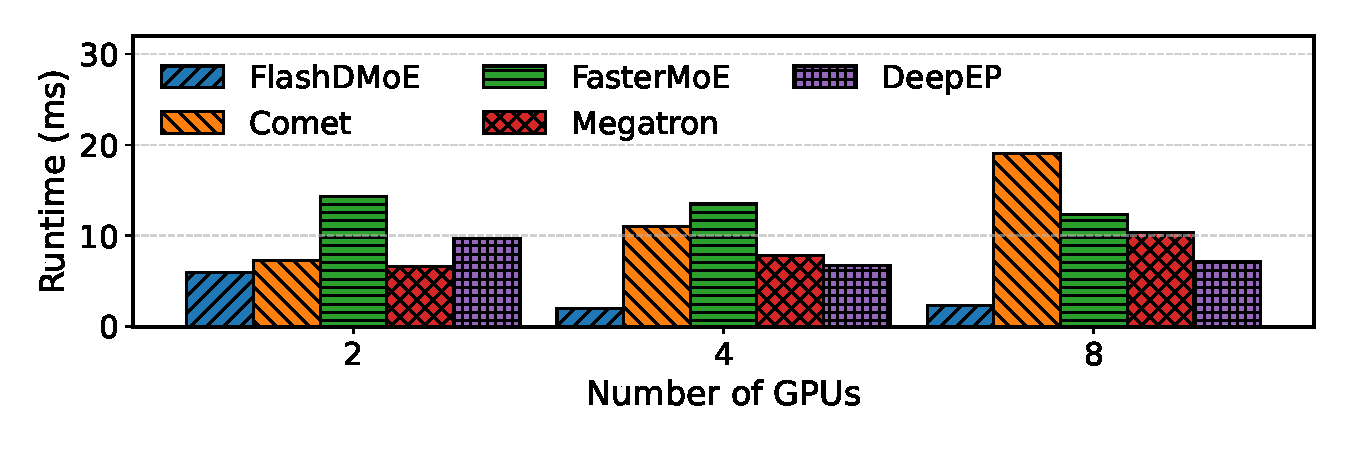
\includegraphics[width=\textwidth, keepaspectratio]{figures/scaling_gpus}
    \caption{Scalability with respect to the number of GPUs (E = 32, T = 8K).}
    \label{fig:scalability-gpus}
\end{figure}
Figure~\ref{fig:scalability-gpus} keeps tokens per GPU constant while scaling GPU count.
\sysname shows strong scalability, achieving a speedup from 5.99 ms (2 GPUs) to 1.98 ms (4 GPUs)
and maintaining performance at 8 GPUs (2.33 ms).
This highlights efficient inter-GPU communication and workload distribution.
Comet and Megatron-LM degrade notably (Comet: 7.26–19.01 ms; Megatron-LM: 6.59–10.32 ms),
indicating communication bottlenecks at scale.
FasterMoE shows modest improvements (14.28–12.37 ms),
and DeepEP displays a similar pattern to \sysname (9.65–7.12 ms) but with consistently higher runtimes.
\section{SM Utilization}\label{sec:sm-utilization}
\begin{figure}[!ht]
    \centering
    \subcaptionbox{Comparison of SM utilization, defined as the ratio of cycles in which SMs have at least one warp in flight to the total number of cycles~\cite{nsight-metrics}. Values represent the average SM utilization over 100 iterations. All experiments use T = 8K and E = 64 on two GPUs.\label{fig:sm-util}}{%
        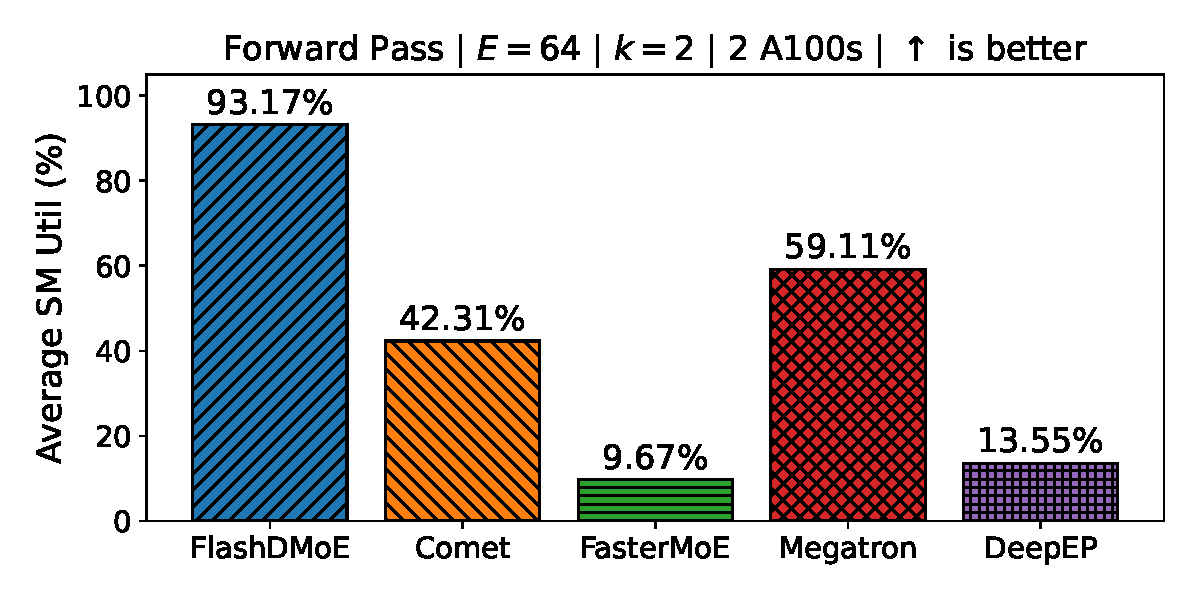
\includegraphics[width=0.7\linewidth]{figures/sm_util}
    }
    \hspace{2pt}
    \subcaptionbox{Payload efficiency. The y-axis shows the total number of bits transferred over NVLink with the same configuration. The x-axis shows the total layer execution time over 100 iterations. Both axes are log-scaled.
    % \byungsoo{Need to make sense of this result: why larger payload size for FasterMoE despite uniform configuration?}
    \label{fig:payload-efficiency}}{%
        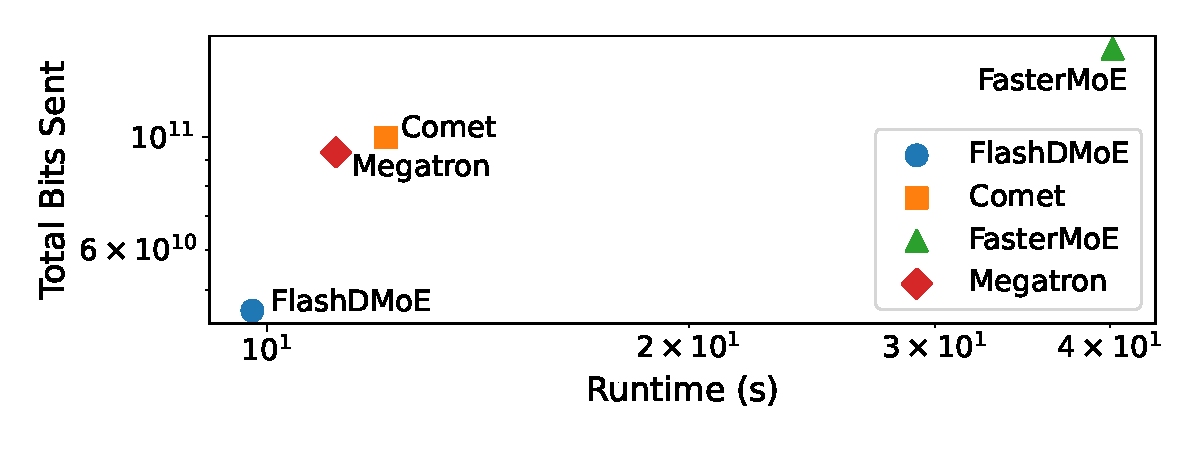
\includegraphics[width=0.7\linewidth]{figures/payload_efficiency}
    }
    \caption{Factors leading to performance improvement of \sysname.}
    \label{fig:sm-util-payload-efficiency}
\end{figure}
Figure~\ref{fig:sm-util} shows GPU utilization,
measured by the average SM utilization (fraction of GPU cycles with active warps~\cite{nsight-metrics}).
\sysname achieves over 90\% SM utilization, showing effective fine-grained task scheduling and reduced idle GPU time.
\section{Payload Efficiency}\label{sec:payload-efficiency}
We next evaluate payload efficiency (Figure~\ref{fig:payload-efficiency})
by measuring the volume of data transferred over NVLink.
Traditional MoE frameworks communicate zero-padded tokens,
inflating network payloads.
In contrast, \sysname's in-place padding approach transmits only active tokens,
reducing communication volume substantially and resulting in better runtime performance.
\section{Multi-Node Evaluation}\label{sec:multi-node-evaluation}
\subsection{Setup}\label{subsec:setup}
In this experiment, we seek to evaluate \sysname in the multi-node setting.
We use 4 nodes, where each node comprises 4 A100 GPUs fully interconnected via NVLink.
Across nodes, each GPU uses a single NIC providing 25 GB/s of bandwidth.
We set the number of experts to be $16$ and assign each GPU to host only one,
so the number of local experts is $1$.
Note that we define MIV formally as follows:
\[
    MIV = \frac{Tokens}{Experts} * local\_{experts} * precision * hidden\_size * 2 * n_{rg}
\]
where $n_{rg}$ is the number of remote peers and the multiplicative
factor of $2$ accounts for communication rounds (dispatch and combine).
$n_{rg} = 12$ for this experiment.
\subsection{Results}\label{subsec:results}
\begin{figure} [!ht]
    \centering
    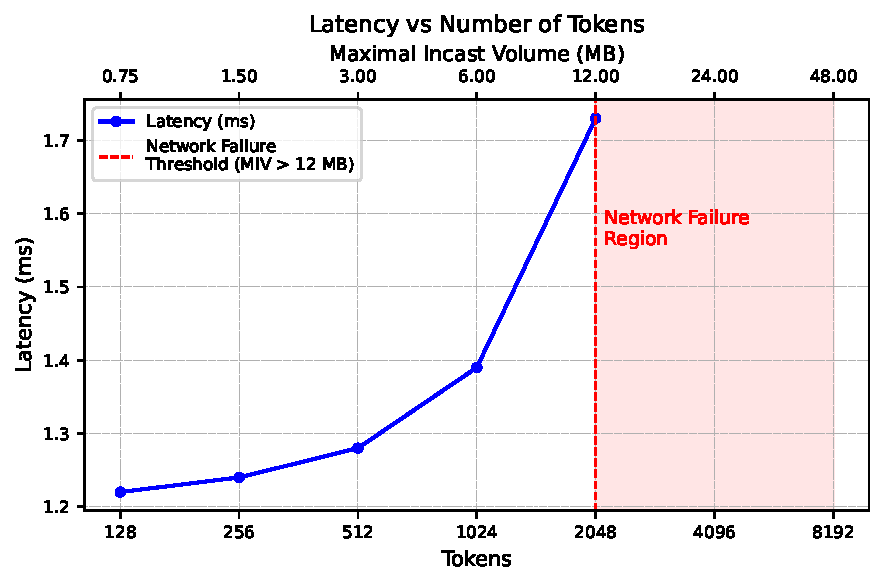
\includegraphics[width=4in,keepaspectratio]{figures/multi_node_fail}
    \caption{Multi-node Latency evaluation.
    Embbeding dimension is $1024$ and FFN intermediate size is $4096$.
    We define Maximal Incast Volume (MIV) as the worst case upper bound for data volume that a
    NIC receives in a single incast occurence.}
    \label{fig:multi_fail}
\end{figure}
We observe a sublinear increase in latency as we scale the number of tokens.
However, we observe at $Tokens > 2048$, that the application fails to terminate
due to failure to receive expectant messages.
We hypothesize this failure to be due to buffer overflow at the networking hardware layer as is common for applications
that generate many and large messages~\cite{nerscNetworkNERSC} like our system.
We note that this failure is addressable by tuning hardware configurations~\cite{ofiwgFi_cxi7} but we consider
this exploration as an exercise orthogonal to this work.
\section{Memory Overhead}\label{sec:eval:memory}
We measure the GPU memory required for the symmetric tensor $L$ and runtime bookkeeping state of \sysname.
Memory overhead depends primarily on the tile size, expert capacity (EC), and the number of experts ($E$).
Table~\ref{tab:memory-overhead} summarizes memory overhead under various configurations,
confirming that \sysname maintains a modest and predictable memory footprint.
\begin{table}[!ht]
    \centering
    \caption{Memory overhead (tile size $bM = 128$, $Size(T) = \text{Tokens} * 4KB$).}
    \label{tab:memory-overhead}
    \setlength{\tabcolsep}{2pt}
    \renewcommand{\arraystretch}{0.9}
    \begin{tabular}{ccccccc}
        \toprule
        \textbf{Tokens} & \textbf{Experts} & \textbf{EC} & \textbf{max(bM, EC)} & \textbf{Bookkeeping (MB)} & $Size(L)$ \textbf{(MB)} & \textbf{Total (MB)} \\
        \midrule
        4K  & 16  & 256  & 256  & 64.57  & 64.00  & 128.57 \\
        4K  & 32  & 128  & 128  & 64.55  & 64.00  & 128.55 \\
        4K  & 64  & 64   & 128  & 128.90 & 128.01 & 256.91 \\
        4K  & 128 & 32   & 128  & 257.96 & 256.02 & 513.98 \\
        \midrule
        8K  & 16  & 512  & 512  & 128.95 & 128.01 & 256.95 \\
        8K  & 32  & 256  & 256  & 128.90 & 128.01 & 256.91 \\
        8K  & 64  & 128  & 128  & 128.90 & 128.01 & 256.91 \\
        8K  & 128 & 64   & 128  & 258.15 & 256.02 & 514.17 \\
        \midrule
        16K & 16  & 1024 & 1024 & 257.89 & 256.02 & 513.90 \\
        16K & 32  & 512  & 512  & 257.79 & 256.02 & 513.81 \\
        16K & 64  & 256  & 256  & 257.80 & 256.02 & 513.81 \\
        16K & 128 & 128  & 128  & 258.53 & 256.02 & 514.54 \\
        \bottomrule
    \end{tabular}
\end{table}
\clearpage
\section{Numerical Data}\label{sec:numerical-data}
\begin{table}[!ht]
    \centering
    \caption{Latency (ms) comparison across different numbers of tokens (Figure~\ref{fig:scalability-token}).}
    \label{tab:latency-tokens}
    \setlength{\tabcolsep}{5pt}
    \renewcommand{\arraystretch}{0.9}
    \begin{tabular}{cccccc}
        \toprule
        \textbf{Tokens} & \textbf{FlashDMoE} & \textbf{Comet} & \textbf{FasterMoE} & \textbf{Megatron} & \textbf{DeepEP} \\
        \midrule
        1024  & 2.07 & 2.87 & 3.85 & 2.59 & 3.80 \\
        2048  & 1.90 & 5.12 & 5.04 & 3.83 & 3.83 \\
        4096  & 2.19 & 9.54 & 7.44 & 5.83 & 4.62 \\
        8192  & 2.33 & 19.01 & 12.37 & 10.32 & 7.12 \\
        \bottomrule
    \end{tabular}
    \vspace{-0.4cm}
\end{table}
\begin{table}[!ht]
    \centering
    \caption{Latency (ms) comparison across different numbers of experts (Figure~\ref{fig:scalability-experts}).}
    \label{tab:latency-experts}
    \setlength{\tabcolsep}{5pt}
    \renewcommand{\arraystretch}{0.9}
    \begin{tabular}{cccccc}
        \toprule
        \textbf{Experts} & \textbf{FlashDMoE} & \textbf{Comet} & \textbf{FasterMoE} & \textbf{Megatron} & \textbf{DeepEP} \\
        \midrule
        16  & 1.20 & 19.01 & 11.38 & 10.47 & 5.59 \\
        32  & 2.33 & 19.01 & 12.37 & 10.32 & 7.12 \\
        64  & 4.20 & 19.21 & 16.64 & 10.47 & 7.49 \\
        128 & 8.20 & 19.36 & 22.65 & 10.47 & 11.30 \\
        \bottomrule
    \end{tabular}
    \vspace{-0.4cm}
\end{table}
\begin{table}[!ht]
    \centering
    \caption{Latency (ms) comparison across different numbers of GPUs (Figure~\ref{fig:scalability-gpus}).}
    \label{tab:latency-gpus}
    \setlength{\tabcolsep}{5pt}
    \renewcommand{\arraystretch}{0.9}
    \begin{tabular}{cccccc}
        \toprule
        \textbf{GPUs} & \textbf{FlashDMoE} & \textbf{Comet} & \textbf{FasterMoE} & \textbf{Megatron} & \textbf{DeepEP} \\
        \midrule
        2 & 6.00 & 7.26 & 14.28 & 6.59 & 9.65 \\
        4 & 1.98 & 10.98 & 13.59 & 7.82 & 6.72 \\
        8 & 2.33 & 19.01 & 12.37 & 10.32 & 7.12 \\
        \bottomrule
    \end{tabular}
    \vspace{-0.4cm}
\end{table}
%! Author = jonathan
%! Date = 5/27/25
\chapter{Limitations and Future Work}\label{ch:limitations-and-future-work}
Despite the performance gains and architectural innovations of \sysname, there are several limitations
worth acknowledging---both practical and conceptual---that open the door to future research.
\begin{itemize}
    \item \textbf{Programming complexity.} Developing fully fused, persistent kernels is a non-trivial engineering task.
    While \sysname proves the feasibility and benefit of such kernels,
    their construction demands deep expertise in GPU architectures,
    synchronization and distributed protocols, and memory hierarchies.
    This high barrier to entry limits adoption.
    Future work may consider compiler-level abstractions or DSLs to democratize this technique.

    \item \textbf{FP16 support and shared memory bank conflicts.}
    \item Although modern GPUs natively support half-precision computation,
    adapting \textsc{FlashDMoE} to FP16 is non-trivial due to shared memory bank conflicts.
    These arise from the mismatch between bank granularity and half-precision
    load-store alignment, leading to degraded memory throughput (\S\ref{ch:fp16-memory-throughput}).
    Overcoming this will require careful rethinking of shared memory access patterns or
    coalesced tile layouts specifically optimized for FP16.

    \item \textbf{Rigid memory allocation.} The current memory allocation scheme used for the symmetric tensor layout
    assumes a static token distribution across experts.
    In reality, expert popularity is often skewed and dynamic.
    Future extensions may explore elastic memory regions or
    runtime-aware reallocation schemes that adapt based on observed routing patterns.

    \item \textbf{Lack of backward pass and training support.} While this work focuses on inference,
    enabling training requires fusing backward computation and gradient communication into the kernel.
    Supporting this entails non-trivial changes to both memory bookkeeping and task descriptor definitions.
    Nevertheless, it remains an exciting direction for extending this system to
    fully support end-to-end training.
\end{itemize}



%! Author = jonathan
%! Date = 5/27/25
\chapter{Conclusion}\label{ch:conclusion}
This thesis introduces \sysname,
the first system to fuse the entire Mixture-of-Experts (MoE)
operator into a single, persistent GPU kernel.
We show that prevailing MoE implementations
suffer from two critical inefficiencies:
(1) CPU-managed synchronous communication that leads to underutilized
interconnects and (2) fragmented execution via multiple GPU kernels,
introducing overhead and synchronization delays.

In contrast, \sysname embraces a model of
GPU autonomy by embedding computation, communication, and scheduling within a unified kernel.
It leverages actor-style concurrency,
warp specialization, and asynchronous (R)DMA to
achieve fine-grained communication–computation overlap.

Our evaluation demonstrates up to \textbf{15$\times$ speedup}
over state-of-the-art systems, up to  \textbf{4$\times$} improved GPU utilization, and
greater payload efficiency, especially in dynamic workloads like MoE.
\sysname challenges the dominant execution paradigms in distributed deep learning
and presents a compelling template for building future GPU-native systems.

While several limitations remain---including programming complexity and lack of FP16 support---this
work lays the groundwork for a new era of \emph{in-kernel distributed computation}.
Future systems may build upon this foundation to enable kernel fusion for
entire training pipelines, ushering in a design shift from CPU orchestration to
\textbf{fully autonomous GPU execution}.
\bibliography{sampleThesis}
\appendix
%! Author = jonathan
%! Date = 5/27/25
\chapter{FP16 Memory Throughput}\label{ch:fp16-memory-throughput}
\begin{figure}[!ht]
    \centering
    \begin{subfigure}{\textwidth}
        \centering
        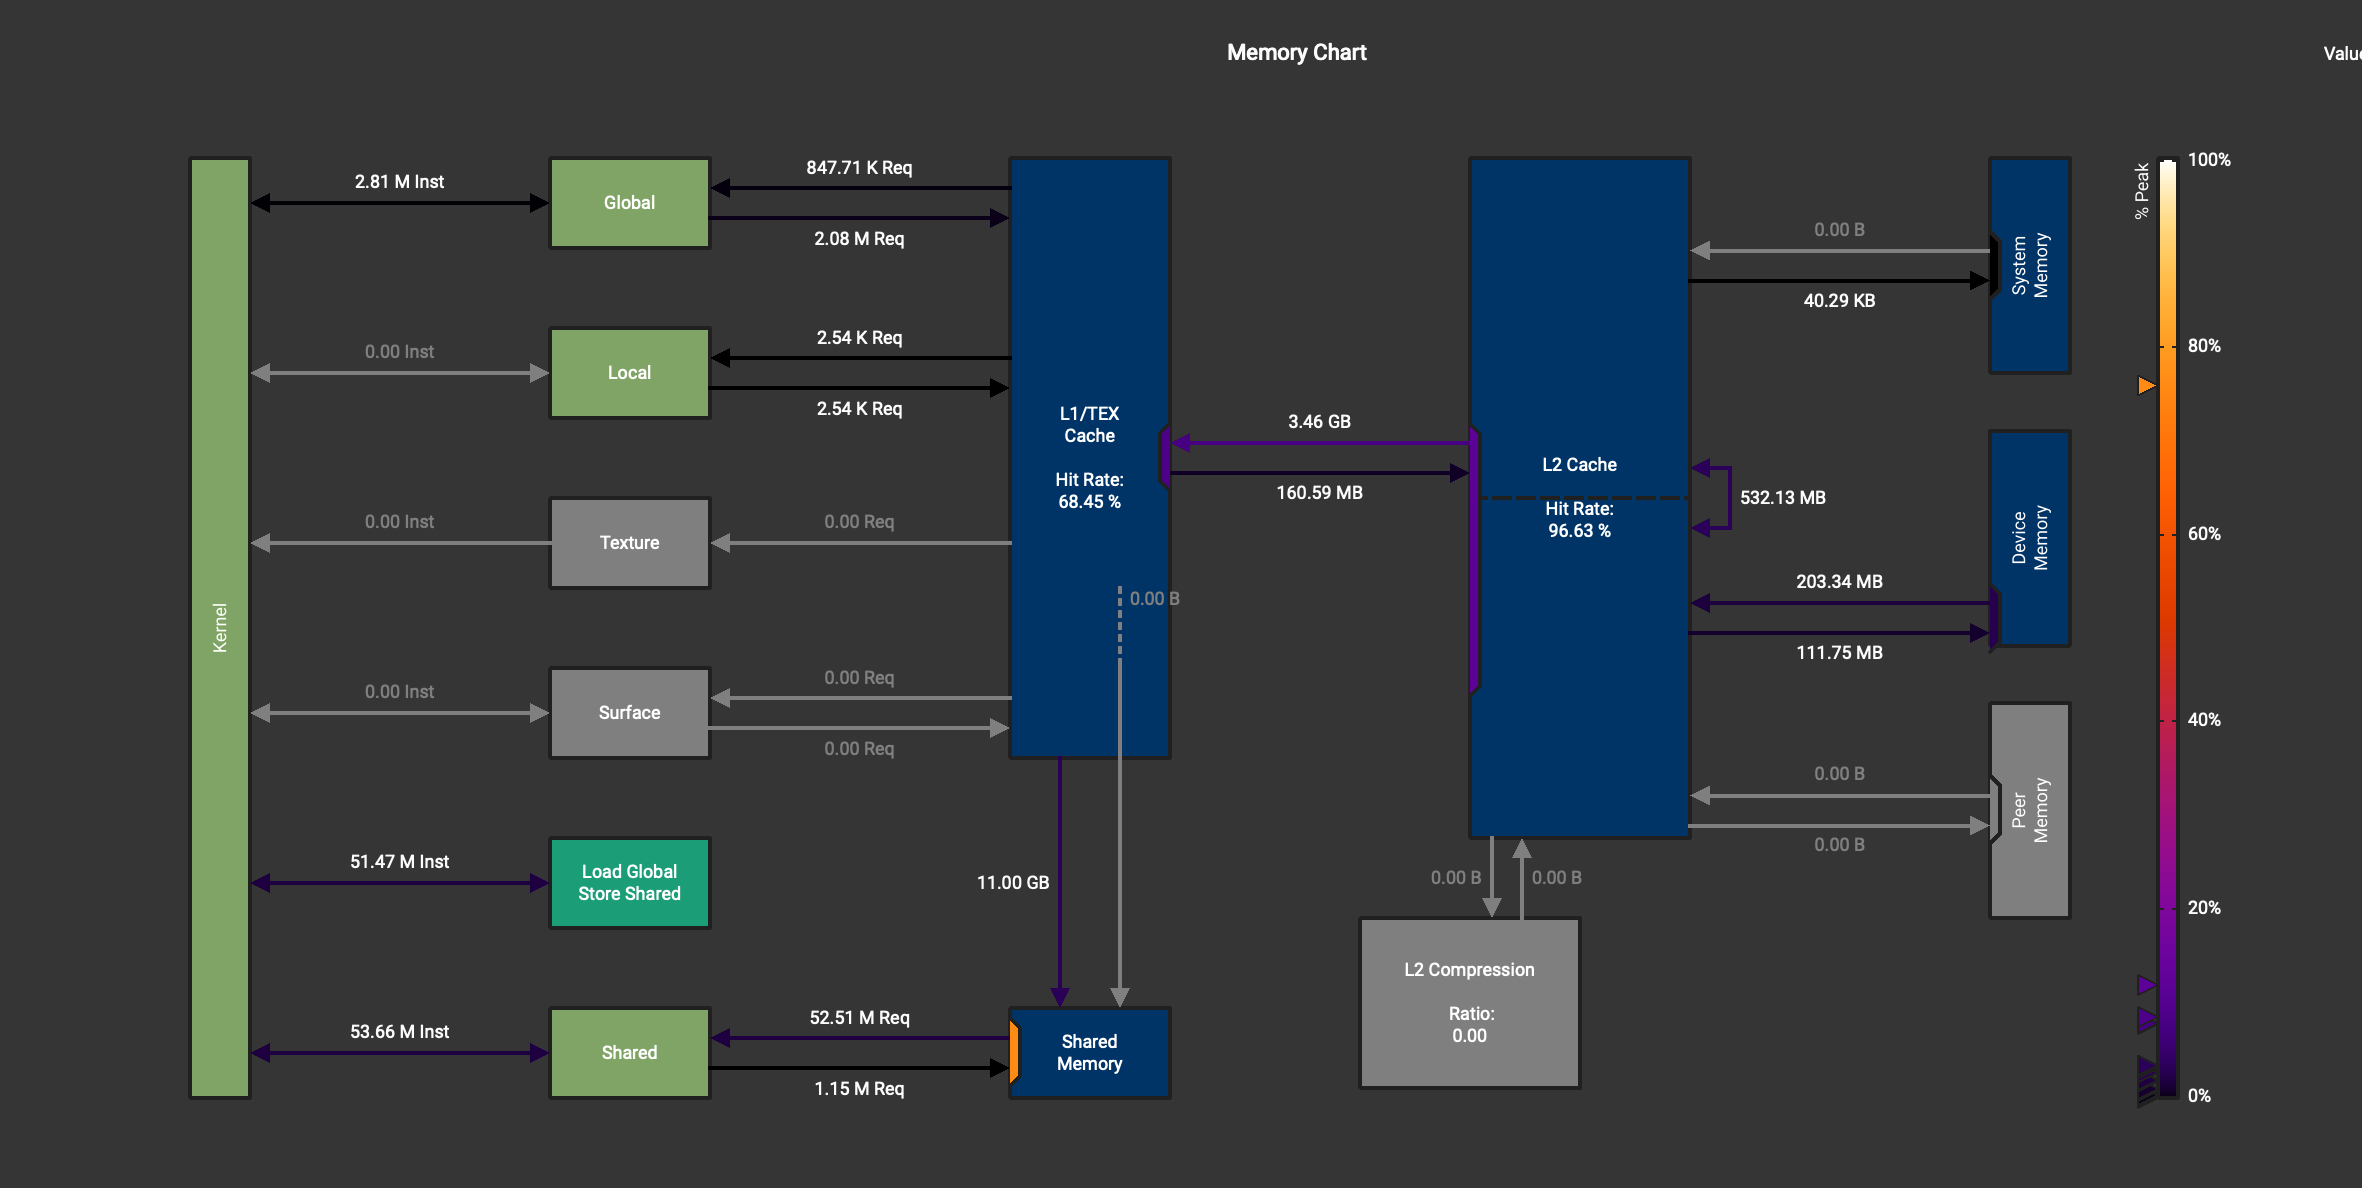
\includegraphics[width=0.9\linewidth, keepaspectratio]{figures/fp16_t}
        \caption{Memory subsystem throughput for FP16}
        \label{sub:fp16}
    \end{subfigure}
    \hfill
    \begin{subfigure}{\textwidth}
        \centering
        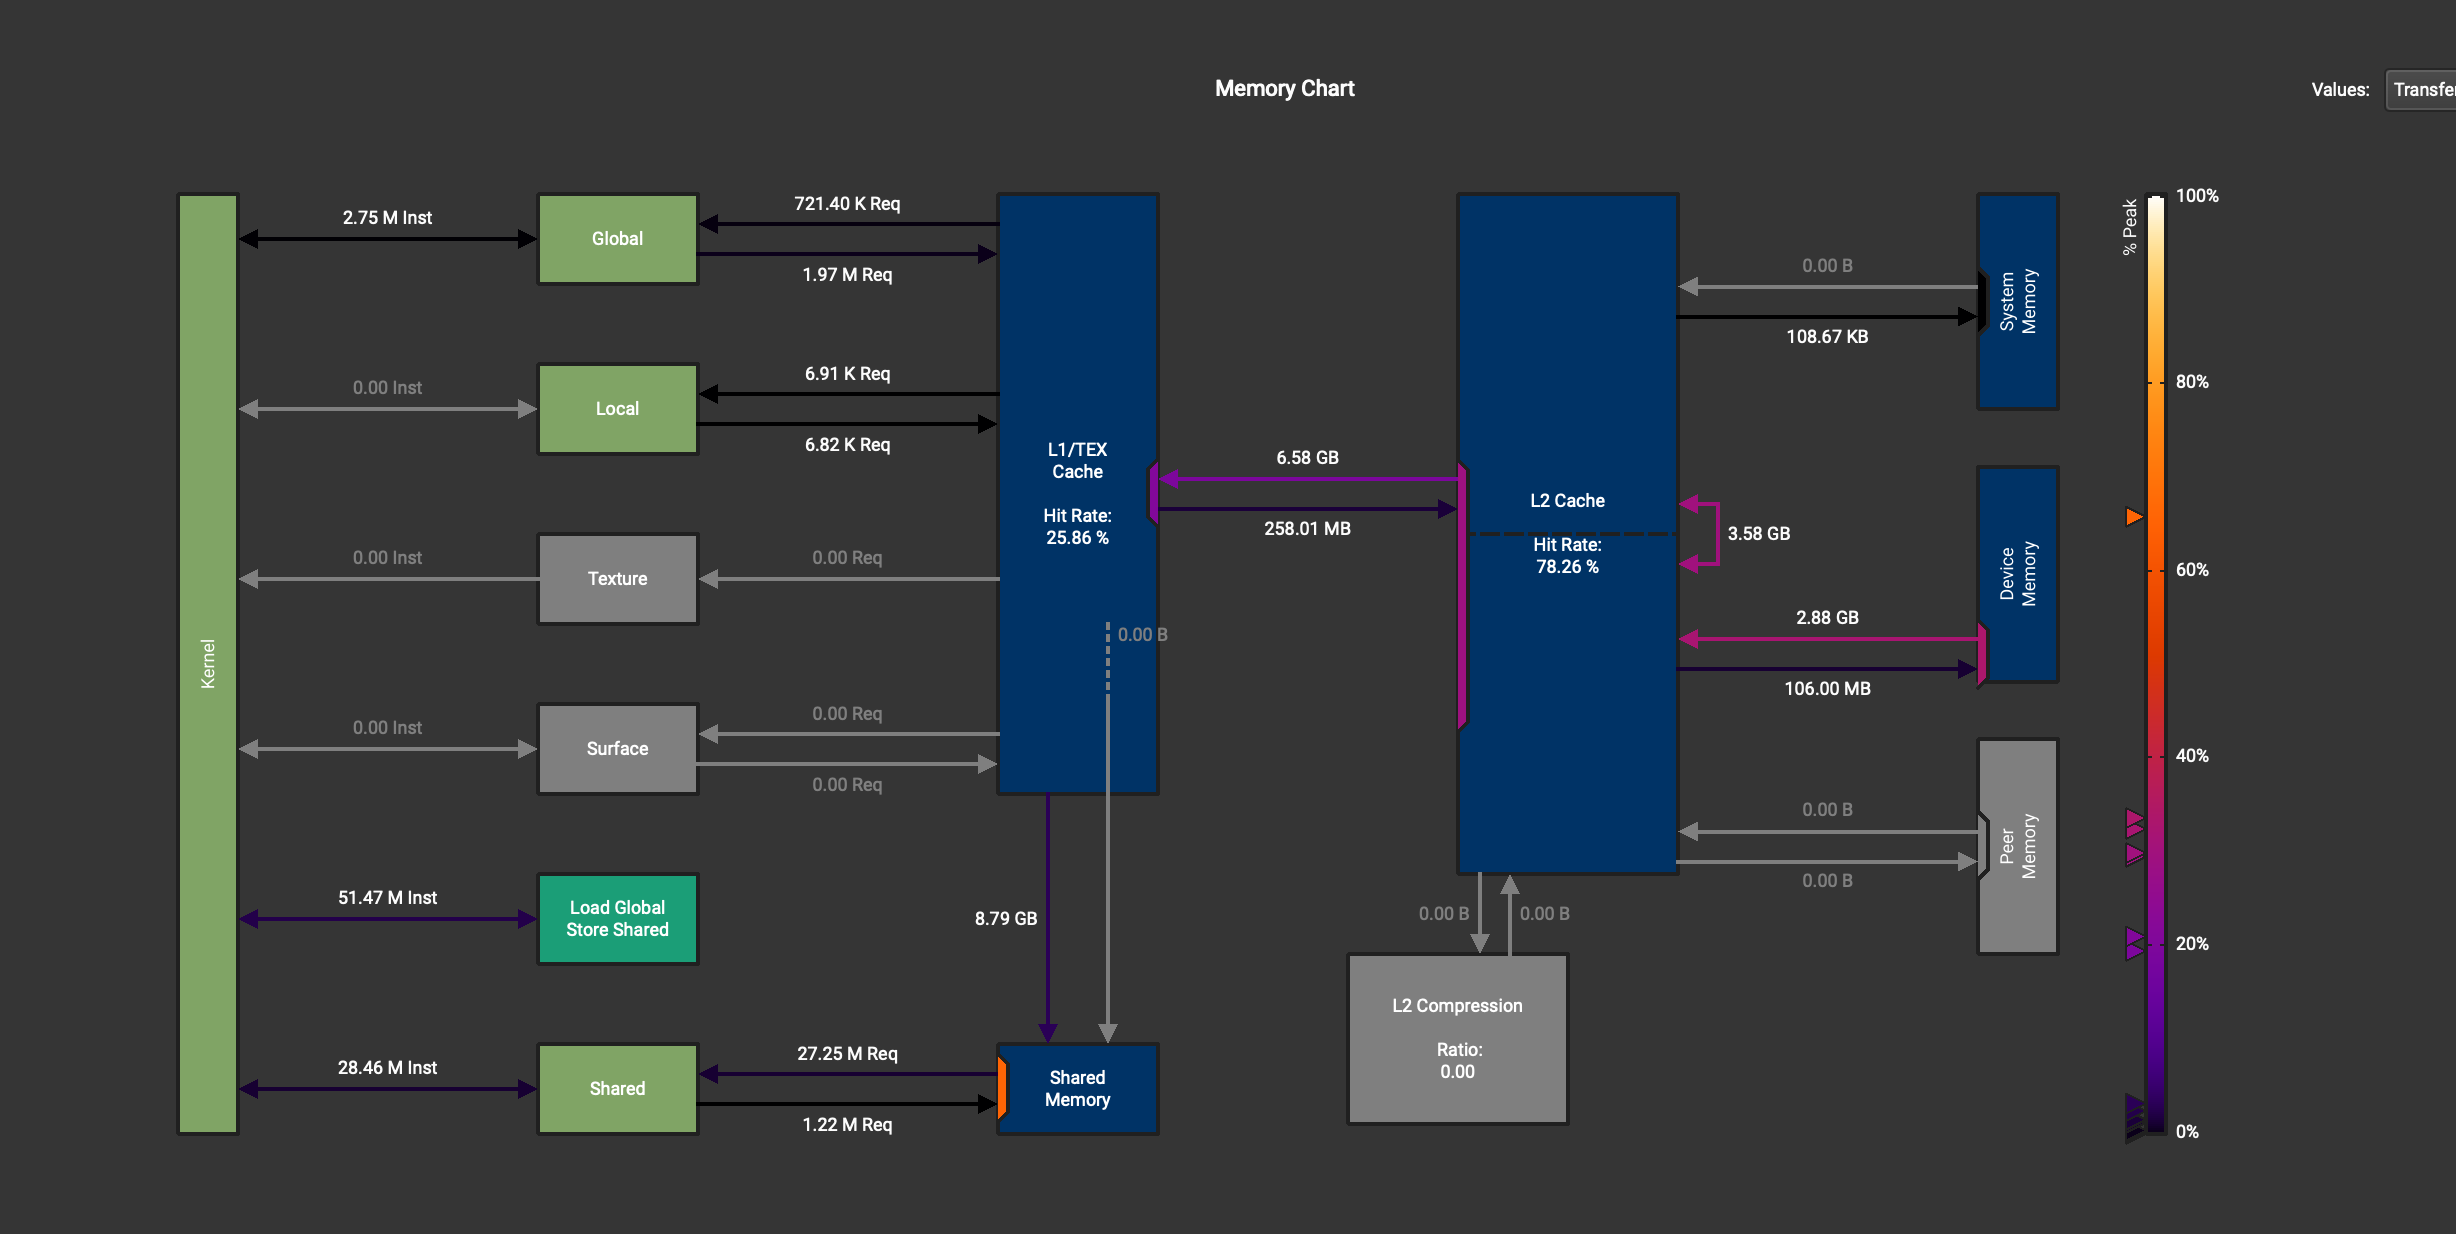
\includegraphics[width=0.9\linewidth, keepaspectratio]{figures/fp32_t}
        \caption{Memory subsystem throughput for FP32}
        \label{sub:fp32}
    \end{subfigure}
    \caption{Here, we report the total GPU memory throughput for both FP16 (top) and FP32 (bottom) variants of \sysname.
    Notably, the FP16 implementation issues approximately $2\times$
        more shared memory instructions compared to its FP32 counterpart
        under identical workloads.
        We attribute this inefficiency to
        suboptimal shared memory layouts in \sysname when
        operating on half-precision data.
        While this bottleneck is addressable through improved layout strategies,
        we leave its resolution to future work due to time constraints.}
    \label{fig:mem_t}
\end{figure}
\end{document}
